%\documentclass[12pt,draftcls]{ucdavisthesis}
\documentclass[13pt,MS]{ucdavisthesis}

% PLEASE READ THE MANUAL - ucdavisthesis.pdf (in the package installation directory)

%%%%%%%%%%%%%%%%%%%%%%%%%%%%%%%%%%%%%%%%%%%%%%%%%%%%%%%%%%%%%%%%%%%%%%%%
%                                                                      %
%               LATEX COMMANDS FOR DOCUMENT SETUP                      %
%                                                                      %
%%%%%%%%%%%%%%%%%%%%%%%%%%%%%%%%%%%%%%%%%%%%%%%%%%%%%%%%%%%%%%%%%%%%%%%%

%\usepackage{bookmark}
\usepackage[us,nodayofweek,12hr]{datetime}
\usepackage{graphicx}
%\usepackage[square,comma,numbers,sort&compress]{natbib}
%\usepackage{hypernat}
% Other useful packages to try
%\usepackage{amsmath}
%\usepackage{amssymb}
%
% Different fonts to try (uncomment only fontenc and one font at a time)
% (you may need to install these first)
%\usepackage[T1]{fontenc} %enable fontenc package if using one of the fonts below
%\usepackage[adobe-utopia]{mathdesign}
%\usepackage{tgschola}
%\usepackage{tgbonum}
%\usepackage{tgpagella}
%\usepackage{tgtermes}
%\usepackage{fourier}
%\usepackage{fouriernc}
%\usepackage{kmath,kerkis}
%\usepackage{kpfonts}
%\usepackage[urw-garamond]{mathdesign}
%\usepackage[bitstream-charter]{mathdesign}
%\usepackage[sc]{mathpazo}
%\usepackage{mathptmx}
%\usepackage[varg]{txfonts}

%To have subfigures
\usepackage{caption}
\usepackage{subcaption}


\hyphenation{dis-ser-ta-tion blue-print man-u-script pre-par-ing} %add hyphenation rules for words TeX doesn't know


%\renewcommand{\rightmark}{\scriptsize A University of California Davis\ldots \hfill Rev.~\#1.0 \quad Compiled: \currenttime, \today}
% a fancier running header that can be used with draftcls options

%%%%%%%%%%%%%%%%%%%%%%%%%%%%%%%%%%%%%%%%%%%%%%%%%%%%%%%%%%%%%%%%%%%%%%%%
%                                                                      %
%        DOCUMENT SETUP AND INFORMATION FOR PRELIMINARY PAGES          %
%                                                                      %
%%%%%%%%%%%%%%%%%%%%%%%%%%%%%%%%%%%%%%%%%%%%%%%%%%%%%%%%%%%%%%%%%%%%%%%%

\title          {Semantic Segmentation of Diseased Rat Brain MR Images over Time}
%Exact title of your thesis. Indicate italics where necessary by underlining or using italics. Please capitalize the first letter of each word that would normally be capitalized in a title.

\author         {Alexander Cyrus Shakouri}
%Your full name as it appears on University records. Do not use initials.

\authordegrees  {B.S. University of California, San Diego 2017}
%Indicate your previous degrees conferred.

\officialmajor  {Electrical and Computer Engineering}
%This is your official major as it appears on your University records.

\graduateprogram{Electrical and Computer Engineering}
%This is your official graduate program name. Used for UMI abstract.

\degreeyear     {2019}
% Indicate the year in which your degree will be officially conferred.

\degreemonth    {December}
% Indicate the month in which your degree will be officially conferred. Used for UMI abstract.

\committee{Jinyi Qi}{Yong Jae Lee}{Soheil Ghiasi}{}{}
% These are your committee members. The command accepts up to five committee members so be sure to have five sets of braces, even if there are empties.

%%%%%%%%%%%%%%%%%%%%%%%%%%%%%%%%%%%%%%%%%%%%%%%%%%%%%%%%%%%%%%%%%%%%%%%%

%\copyrightyear{2020}
%\nocopyright

%%%%%%%%%%%%%%%%%%%%%%%%%%%%%%%%%%%%%%%%%%%%%%%%%%%%%%%%%%%%%%%%%%%%%%%%

\dedication{\textsl{I would like to dedicate this thesis to my parents, Jessie and Mohammed Shakouri. They have supported me all my life and without them I would not be where I am now. }}

%%%%%%%%%%%%%%%%%%%%%%%%%%%%%%%%%%%%%%%%%%%%%%%%%%%%%%%%%%%%%%%%%%%%%%%%

\abstract{
\par
Semantic Segmentation of brain MR images has always been a very time consuming task in the medical industry.
The automation of semantic segmentation will not only help cut down on the time significantly but help reduce intra-observer and inter-observer variability in the MR images. 
The main challenge to automate semantic segmentation is the intra-observer and inter-observer variability as this is what causes the segmented regions to be inconsistent which in turn makes it hard to segment. 
It is also very difficult to get a lot of data for semantic segmentation because it is so time consuming.
Recent advances in deep convolutional neural networks in semantic segmentation of natural and medical images allows for the mitigation of these challenges. 
\par
This thesis will utilize deep convolutional neural networks to automate the semantic segmentation of diseased rat brain MR images that vary over time. 
The model will take into account not only healthy rats, but rats with seizures induced and rats with seizures induced but given anti-seizure drugs. 
This complicates the automatic segmentation further as the rat brain images themselves vary significantly between diseased rats and healthy rats and create a spectrum that the model would have to take into account. 
This thesis will investigate multiple different deep convolutional neural networks that have had success in semantic segmentation and apply them to the rat brain MR images.
We will first consider single region segmentation results and how well the models perform on the rat brain images in general.
In the second part of the thesis, the models are applied to semantically segment the MR image into 14 different brain regions.
\par
In the experiments, the segmentation results on rat brain MR images is shown as well as the training and validation curve for the corresponding model. 
The models experimented are U-net, dilated convolution models, and a combination of both at multiple downsampling levels. 
The experimental results show that the combination of U-net and the dilated models at 3 downsampling layers performed the best with an average dice score of 0.812 from healthy to diseased rats.
The results also show that automatic segmentation by the deep convolutional neural networks was comparable to the manual segmentation of the rat brain MR images by a trained physician. 
Further work to use 3D convolutional neural network models or multiple MR modalities as an input would help strengthen the results of the model.
}

%%%%%%%%%%%%%%%%%%%%%%%%%%%%%%%%%%%%%%%%%%%%%%%%%%%%%%%%%%%%%%%%%%%%%%%%

\acknowledgments{I would like to express my sincerest gratitude to my major professor Jinyi Qi.
He is an amazing advisor who consistently tries to help his students in every way possible.
I really appreciate his patience when going through the experimental results and he always provided essential input for this thesis.
He really inspired me to try to figure things out on my own, but of course he would be there if I needed help with anything. 
Thank you so much for everything and I really appreciate everything you have done for me.
\par
I would also like to thank everyone else who helped me with writing this paper. 
I would like to thank my other committee member professors as well, Yong Jae Lee and Soheil Ghiasi for helping me with my research and completing this thesis.
Thank you so much for being part of my thesis committee and for discussing my research.
Thank you Brad Hobson and Doug Rowland for helping to provide the rat brain MR images as well as starting this research. 
I really appreciate how excited you were at this research and for preparing the ground truths for my use.
\par
I would finally like to thank everyone in my research group as well: Xuezhu Zhang, Chih-Chieh Liu, Zhaoheng Xie, Reheman Baikejiang, Mengxi Zhang, TianTian Li, and Nimu Yuan. 
You all helped me feel so welcome in the lab and always were very helpful. 
I really enjoyed being lab mates with you all and I wish you all the best. 
}

%%%%%%%%%%%%%%%%%%%%%%%%%%%%%%%%%%%%%%%%%%%%%%%%%%%%%%%%%%%%%%%%%%%%%%%%

% Each chapter can be in its own file for easier editing and brought in with the \include command.
% Then use the \includeonly command to speed compilation when working on a particular chapter.
%%% \includeonly{ucdavisthesis_example_Chap1}

\begin{document}

\newcommand{\bibfont}{\singlespacing}
% need this command to keep single spacing in the bibliography when using natbib

%\bibliographystyle{unsrtnat}
\bibliographystyle{IEEEtran}
%many other bibliography styles are available (IEEEtran, mla, etc.). Use one appropriate for your field.

\makeintropages %Processes/produces the preliminary pages

\chapter{Introduction}
%l
Semantic segmentation is the task of predicting regions across the entire image \cite{DBLP:journals/corr/abs-1809-10198semanticprogress}. 
It is known as pixel-level segmentation because every pixel of the image is associated with a class. 
Semantic segmentation is a problem where you need not only pixel wise accuracy, but multi-scale context as well \cite{Yu2016MultiScaleCA}. 
This is due to the fact that we need to use the multi-scale context in order to predict correctly at the pixel level. 
For example a horse in an image has many pixels associated with it, but one would need to know what a horse looks like in order to correctly predict each pixel in the image. 
This problem has been discussed extensively for natural images \cite{DBLP:journals/corr/LongSD14}, \cite{DBLP:journals/corr/ChenPSA17}, \cite{Yu2016MultiScaleCA} as well as for medical images \cite{DBLP:journals/corr/RonnebergerFB15}. 
There are many applications for semantic segmentation outside the medical field, such as for autonomous driving \cite{inbookautomous}, facial segmentation \cite{7350915face} and many other applications. 

The medical imaging field has a great use for autonomous semantic segmentation because segmenting medical images is a time consuming task for doctors.
In order to get a good segmentation a doctor not only needs great expertise in the forming of the regions, but also needs to take the time to manually draw it out, when they are busy with many other tasks.  
Autonomous semantic segmentation will help reduce the time it takes to fully segment a medical image drastically with the doctors only having to spend time to study the image for the patient.
This will also aid doctors not only in the diagnosis of the patient, but also help to standardize the process so that fatigue or human error does not affect the results of the segmentation \cite{SharmaAutomatedImageSegmentationTech}. 
This thesis will focus on the task of semantic segmentation of the brain, specifically rat brain MRI's.
This thesis proposes an implementation of the most popular methods for semantic segmentation and applies it to rat brain MRI's taken over time. 


\section{MR images}
        Magnetic Resonance Imaging or MRI is a radiology technique that produces three dimensional anatomical images. 
        MRI utilize a strong magnetic field as well as radio waves in order to measure the energy released from atoms realigning with the magnetic field \cite{doi:10.1002/9781118786574.ch1MRI}. 
        Different types of tissue have different magnetic properties and so using the MRI technique we are able to differentiate them within the image. 
        MRI is a type of anatomical imaging where the goal is to create an accurate visual representation of the tissues being imaged. 
        Doctors are able to use MRI images for many purposes, for example to diagnose diseases or to see any abnormalities in a person's body. 
        There also also multiple different sequences for MRI's that correspond to different types of tissue being more excited than others.
        Some of the most common sequences are T1 weighted, T2 weighted, and Flair where each one corresponds to different tissues being excited more than others. 
        This thesis will just focus on T2 weighted MRI's.
        MRI of the brain is usually taken in a 3D volume. 
        Each MRI will consist of a x,y, and z dimensions corresponding to a series of 2D images.
        The reason that it can correspond to a series of 2D images is that the voxels in the MRI are not necessarily evenly spaced in different dimensions. 
        Usually the z dimension is differently spaced than the x,y dimensions, but it depends on a number of factors including MRI magnet strength, imaging parameters, etc.
        
\begin{figure}
\centering
\begin{subfigure}{.5\textwidth}
  \centering
  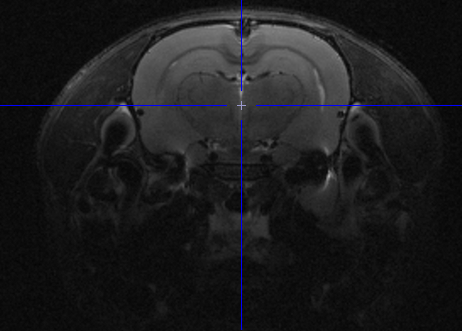
\includegraphics[width=.6\linewidth]{coronal_brain_view.png}
  \caption{Coronal slice of a rat brain}
  \label{fig:coronal}
\end{subfigure}%
\begin{subfigure}{.5\textwidth}
  \centering
  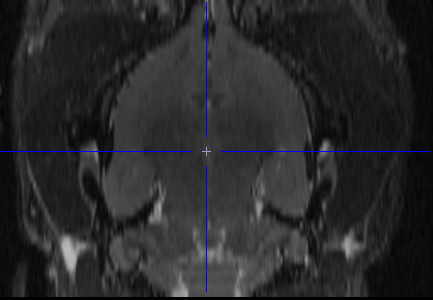
\includegraphics[width=.6\linewidth]{axial_brain_view.png}
  \caption{Axial slice of a rat brain}
  \label{fig:axial}
\end{subfigure}
\begin{subfigure}{.3\textwidth}
  \centering
  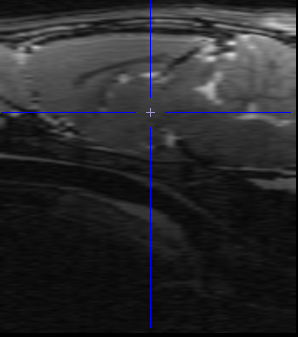
\includegraphics[width=.6\linewidth]{sagittal_brain_view.png}
  \caption{Saggital slice of a rat brain}
  \label{fig:saggital}
\end{subfigure}

\caption{This figure shows an example of the data that will be used in this thesis. They are T2 weighted MRI images of size 280x200x44. }
\label{fig:MRI image}
\end{figure}

\section{Statement of Problem}
        This thesis will introduce an automatic method to segment MRI rat brain images into 14 different regions for quantification studies. 
        The data used in this thesis is provided by the CMGI or the Center for Molecular or Genome Imaging and consists of rat brain T2 wieghted MR images. 
        The study imaged 40 total different rats at three separate time points; day 3, day 7, day 28. 
        This study was conducted to learn more about the effects of anti-seizure drugs.
        The rats were given Diisopropyl fluorophosphate or DFP to induce seizures. 
        Some rats were also given anti-seizure drugs, Midazolam (MDZ) or Diazepam (DZP) and imaged to compare the effects of the drugs.
        This thesis will focus on implementing an autonomous method that can segment multiple regions in MR images. 
        The 40 animals were split up in multiple groups in order to effectively test the drugs.
        The dataset was split into 10 animals for the the control group or vehicles (VEH), 10 animals that are given DFP and basic treatment, 10 animals that are given DFP and then MDZ, and 10 animals that are given DFP and DZP. 
        Each one of these animals had MR images taken at three different time points mentioned above for a total of 120 scans. 
        Each one of these scans was semantically segmented by two people who tried to stay as consistent as possible. 
        The ground truth consists of 14 different regions most pertaining to areas in the brain as shown in figure ~\ref{fig:segmentation regions}. Each left and right region will be split into its corresponding left and right sides of the brain except for the medial thalamus. The cerebellum is also segmented but not shown in the figure ~\ref{fig:segmentation regions} making the total regions segmented 14. 
        
\begin{figure}
  \centering
  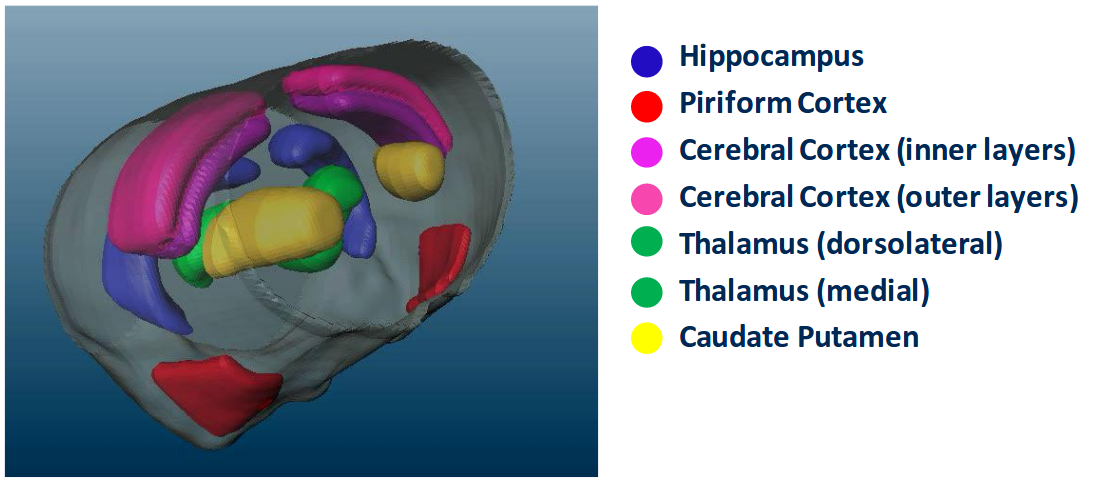
\includegraphics[width=\linewidth]{segmentation_areas.png}
  \caption{MRI rat brain segmentation regions relative to the brain. Image provided by Brad Hobson. }
  \label{fig:segmentation regions}
\end{figure}
        
\section{Challenges} 


    Semantic segmentation has been implemented successfully with the invent of deep neural networks.
    The medical field has a great need for semantic segmentation, but the availability for medical images to train on is usually scarce, compared to the thousands or millions of images available in the natural world.
    This makes the task of semantic segmentation much harder when applied to the medical field as when it comes to training deep neural networks data is essential. 
    
    There are many problems associated with segmentation segmentation, especially when it applies to the medical industry. 
    One of the main problems is that models can't be trained with millions of images like in the natural image case. 
    It is very hard to obtain a large data set when it comes to medical images because of privacy laws as well as just general availability of the images. 
    It is much easier to find many different images and its segmentation of a horse than a brain. 
    Before the medical images can be used in models it has to have no connection with the 
    A lot of the time the images being gathered have personal data attached to it and so before the data can be used into a model all information that can be used to identify it has to be removed. 
    
    Another big challenge is that getting the ground truths of the data is very time consuming. 
    In order to be able to accurately segment an image of the animal, one needs to be an expert in that animal. 
    It is not common knowledge to know how to segment the different regions in a brain versus the segmentation of a horse.
    There are no clear boundaries in some regions of the brain and so a lot of the time experts will segment the regions slightly differently. 
    This makes it so there are larger inter-observer and intra-observer variability in medical imaging than in natural images. 
    
    Inter-observer and intra-observer variability is one of the main challenges of medical imaging segmentation.
    The VEH or control group stays the most consistent whereas the DFP group after a certain amount of time the brain region even for the same animal will have vastly different segmented regions.  
    This is due to brain loss and other complications due to the induced seizure that the rats go through.  
    
 

\section{Outline}
    This thesis will first review in detail some existing methods for semantic segmentation in chapter 2. 
    Chapter 3 will be focused on our approach to semantic segmentation issue. 
    Chapter 4 will discuss the data in more detail and how we utilize it in our models. Chapter 5 will discuss the results and finally in Chapter 6 we will conclude the work of this thesis and discuss the future directions.
\chapter{Related Works}


\section{Neural Networks}
    Neural networks are the most widely used method for many different applications including semantic segmentation. 
    Neural Networks are used to map a non-linear input to an output. 
    A neural network is made up of its input layer, any number of hidden layers and an output layer \cite{DeepLearning2015}.
    Neural networks are inspired after neurons in the brain \cite{DeepLearning2015}, \cite{Goodfellow-et-al-2016}, \cite{10.1371/journal.pcbi.Neurons}. 
    Each element within the vector of the input layer can be seen as a "neuron" where each element is interconnected and takes the information before it to make a decision and send it to another "neuron".
    This makes it so that as the layers go deeper in a neural network, the neurons are able to learn more and more complex things from the previous neurons.
    \par
    The input layer consists of the input for the task the network is supposed to learn. 
    For example for the image classification and segmentation tasks, usually the input would be the image the network is supposed to classify. 
    The hidden layers can be seen as a function that tries to predict the output. 
    Each hidden layer applies a function to the previous layer; each subsequent hidden layer is able to predict a more complex function.
    The output of the first and hidden layers is a feature map that the model will use in the subsequent layer \cite{Goodfellow-et-al-2016}. 
    The output layer finally consists of the probabilities associated with the final output 
    For example for image classification the output layer would be associated to a probability for each class, while for semantic segmentation, each pixel would have a probability associated with it for each class. 
    A basic neural network is shown in figure ~\ref{fig_neuralNetwork}. 
    
    
\begin{figure}[tbh]
\centering
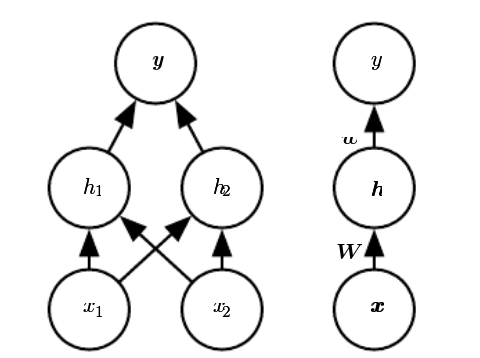
\includegraphics[width=\textwidth]{neural_network.png}
% where an .eps filename suffix will be assumed under latex,
% and a .pdf suffix will be assumed for pdflatex
\caption{This is an example of a neural network. On the right we see the basic outline of the network with the input layer at the bottom with x, the hidden layer represented by h, and the output layer represented by y. Along each arrow is a W or a weight associated with the output of the previous layer. On the left shows a vectorized view of the right where each layer can have multiple elements. Image is from \cite{Goodfellow-et-al-2016}.}
\label{fig_neuralNetwork}
\end{figure}    


\subsection{Convolutional Neural Networks}
Convolutional Neural Networks or CNN's have had huge success with the task of semantic segmentation \cite{Girshick_2014_CVPR}, \cite{Long_2015}. 
Convolutional Neural Networks are one type of Neural Network, but a convolutional layer receives its input from multiple output nodes.
This allows convolutional neural networks to capture local information. 
The output of these convolutional layers is a feature map of the previous layer which takes a linear combination of the input to that layer \cite{Lee:2011:ULH:2001269.2001295}.
This allows for the model to learn complex shapes and use them to get the correct final output. 
The features that the convolutional neural network will learn depend on the task the network is trained for.
Figure ~\ref{fig:feature_map} shows the feature maps for a convolutional neural network trained on the segmentation of a region in an image. 
Figure ~\ref{fig:first_feature} show the output of 24 different filters of the first layer of a neural network trained on. Figure ~\ref{fig:second_feature} show the output of 100 different filters created from a linear combination of any number of filters in the first layer. 
This can be seen as in the first layer the feature maps are straight or curved lines usually, but for the second layer there are also circles or multiple different lines within the feature map.
The network learned straight or curved lines in the first layer or more complex shapes in the second layer as the network was trained to segment an image.
It is beneficial to increase the number of filters as we go deeper in the network so that the model can use more combinations of the previous layers features. 
There is no standard for the exact number of features one should use in a model as it depends on the task and how much the network would have to learn.

\begin{figure}
\centering
\begin{subfigure}{.5\textwidth}
  \centering
  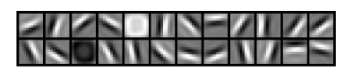
\includegraphics[width=.6\linewidth]{first_layer_features.png}
  \caption{Feature map of first layer in convolutional neural network}
  \label{fig:first_feature}
\end{subfigure}%
\begin{subfigure}{.5\textwidth}
  \centering
  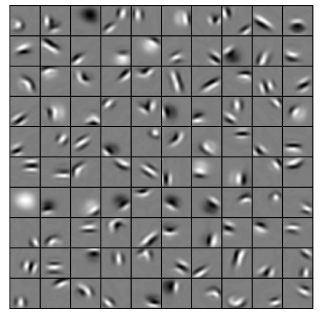
\includegraphics[width=.6\linewidth]{Second_layer_features.png}
  \caption{Feature map of second layer in convolutional neural network}
  \label{fig:second_feature}
\end{subfigure}
\caption{This network was trained on the segmentation of an image. The feature maps of the first and second layers are shown above. The features of the second layer are a linear combination of the features in the first layer. }
\label{fig:feature_map}
\end{figure}
    
\subsubsection{Convolution}
    Convolution is the element wise multiplication and addition of an image and a kernel. 
    Let $L:Z^2 \rightarrow R $ be a discrete function. 
    Let f be a discrete filter of size $(2r+1)^2 $. 
    The convolution operation $*$ can be shown as
\begin{equation}
 (L * f)(s) = \sum_{n+p=s}\sum_{m+p=s} L(m,n)f(p)\label{eq:convolution}
\end{equation}
    
    An example of this is shown in ~\ref{fig_convolutionOperation}. 
    The input is the image or feature map from a previous layer while the kernel matrix is the weight matrix learned by the model. 
    Each output pixel or feature map is calculated by the dot product of the kernel and appropriate image patch and then is moved across the image one pixel at a time. 
    This movement of the kernel across the image is called the stride and is usually 1 in order to not miss any important features that the model might see and get the best performance \cite{pmlr-v15-coates11a}. 
    Usually the kernel used is much smaller than the image in question in order to have sparse connections.
    This leads the model to learn small meaningful features as the output \cite{Goodfellow-et-al-2016}. 
    In convolution layers the kernel matrix is held constant so as to prevent over fitting and ease training. 

\begin{figure}[tbh]
\centering
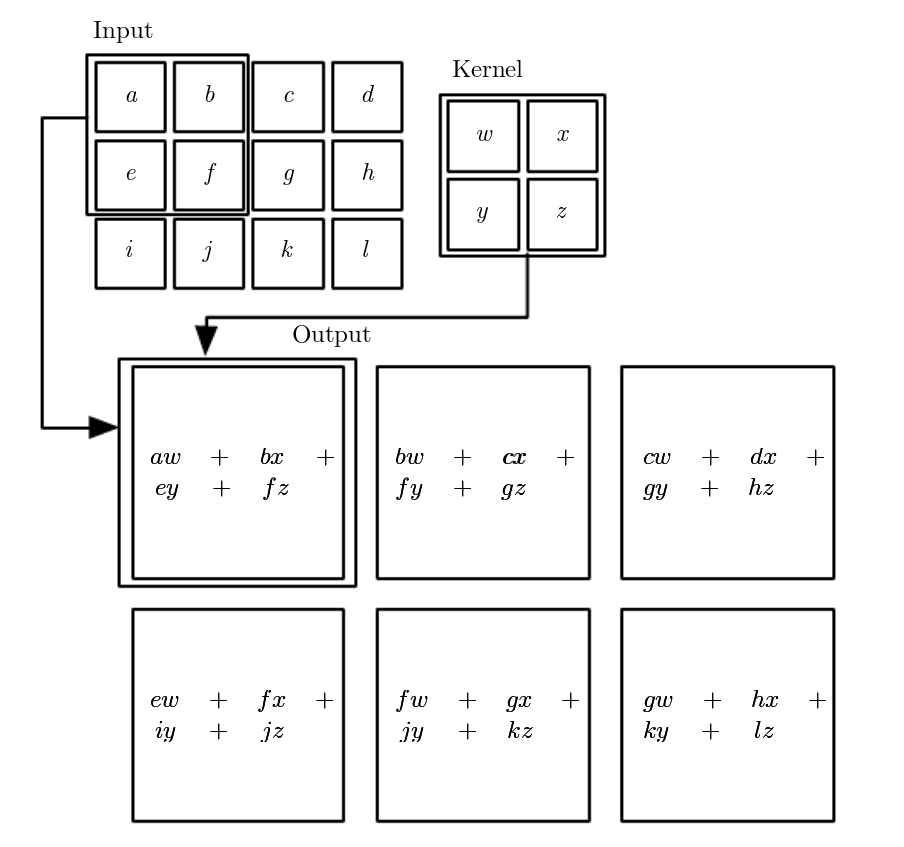
\includegraphics[width=\textwidth]{convolution_operation.png}
% where an .eps filename suffix will be assumed under latex,
% and a .pdf suffix will be assumed for pdflatex
\caption{This is an example of the convolution operation as it is applied to images. Image is from \cite{Goodfellow-et-al-2016}.}
\label{fig_convolutionOperation}
\end{figure} 


\subsubsection{Dilated Convolution}
    Dilated convolutions are different from regular convolutions because they apply the same convolutional filter at different receptive field sizes according to the dilation rate \cite{Yu2016MultiScaleCA}.
    The filter applied to the input has spaces in between the elements corresponding to the dilation rate.
    If we take the convolution operator definition and add $d$ be the dilation factor then the convolution operation can be shown as 
\begin{equation}
 (L *_d f)(s) = \sum_{m+dn=s} L(m)f(n)\label{eq:dilconvolution}
\end{equation}

     According to the dilation rate the filter is applied to different parts of the image, increasing the receptive field size \cite{DBLP:journals/corr/ChenPSA17}. 
     If we define $i$ to be the dilation factor then we can define the filters with increasing dilation as
    
\begin{equation}
 L_{i+1} = L_{i*2^i} f \qquad \mbox{for   } i = 0,1,...,n\label{eq:dilatedrate} 
\end{equation}
    
    An example of three different types of dilation are shown in figure ~\ref{fig_dil_convolution}.
    As the dilation rate increases the receptive field size increases by $(2^{i+2}-1)$x$(2^{i+2}-1)$ where $i$ corresponds to the dilation factor.
    The dilation can be computed by $2^i$ where $i$ is the dilation factor ranging from 0 to n. 
    Dilated convolutions allow the receptive field size to increase exponentially without losing image resolution.
    Regular convolutional layers would need to go much deeper in order to get the receptive field size that dilated convolutions can have.
    
\begin{figure}[tbh]
\centering
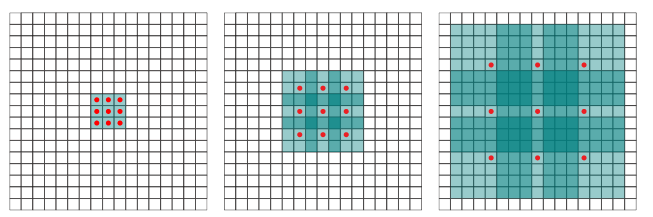
\includegraphics[width=\textwidth]{dilated_convolutions.png}
% where an .eps filename suffix will be assumed under latex,
% and a .pdf suffix will be assumed for pdflatex
\caption{This is an example of how the receptive field size increases with dilation rate. The first image on the left shows a dilation of 1 which corresponds to a dilation factor of 0 and is a normal kernel applied to the input and has a receptive field size of 3x3. The second image shows a dilation of 2 or dilation factor of 1 applied to the input and correspondingly a receptive field size of 7x7. The last image shows a dilation of 4 or dilation factor of 2 applied to the input with a receptive field size of 15x15. Image is from \cite{Yu2016MultiScaleCA}. }
\label{fig_dil_convolution}
\end{figure}     

\subsection{Activation Functions}    
    Neural networks not only need convolutional layers, but activation functions in order do a lot of the tasks we need.
    This is because without activation functions the model would just be a huge linear model, which while useful is not able to account for more complex cases.
    Activation functions help to add a non linearity to the neural network to help it learn more complex tasks.
    Many different types of activation functions have been used in the history of neural networks. 
    The standard was to use $f(x) = tanh(x)$  or sigmoid, $f(x) = 1/(1+e^{-x})$, as the output function for every layer. 
    It was later proved that ReLu or Rectified Linear Units actually trained convolutional neural networks several times faster \cite{NIPS2012_Krizhevsky}. ReLu also was proven to approximate all functions dimension n as long as the width of the network was greater than n \cite{NIPS2017_ReLuUniversalTheorem}. 
    ReLu is a nonlinear function defined as $f(x) = max(0, x)$. 
    This simple function allowed for faster training time because the tanh function saturates after a certain point as seen in figure ~\ref{fig:activation}. 
    This means that for values farther from zero the values will barely change. 
    This is fixed with ReLu as it never fully saturates which allows for easier training. 
    ReLu also preserves some of the linearity which allows for easier optimization and better generalization \cite{Goodfellow-et-al-2016}. 
    This thesis uses ReLu activation function for all the convolution layers.

\begin{figure}
\centering
\begin{subfigure}{.5\textwidth}
  \centering
  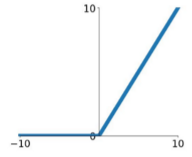
\includegraphics[width=.6\linewidth]{ReLu.png}
  \caption{plot of ReLu function $f(x) = max(0,x)$}
  \label{fig:ReLu}
\end{subfigure}%
\begin{subfigure}{.5\textwidth}
  \centering
  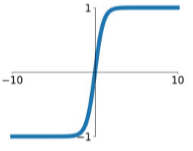
\includegraphics[width=.6\linewidth]{tanh(x).png}
  \caption{plot of tanh function $f(x) = tanh(x)$.}
  \label{fig:tanh}
\end{subfigure}
\caption{This figure shows some common activation functions.}
\label{fig:activation}
\end{figure}

\subsection{Pooling}
    Convolutional layers with non linear activation functions are not enough for models to learn well. 
    Whenever there are convolutional layers most of the time there are also layers that shrink the representation of the convolutional layers as it greatly helps the model train \cite{Lee:2011:ULH:2001269.2001295}. 
    Pooling just takes a small subsample of the input and combines it into one pixel output. 
    The size of the subsampled input is determined by the filter size of the pooling layer. 
    A 3x3 filter will take 3x3 inputs and output a 1x1. 
    The pooling function would then be applied to the entire output using a sliding window. 
    Pooling layers help the model learn spatial invariance as well as reduce the dimensionality of the feature map \cite{Scherer:2010:EPO:1886436.1886447}. 
    Average pooling was widely used in the start of invent of convolutional neural networks \cite{NIPS2012_Krizhevsky}. 
    Average pooling applies the average function to the subsample input and outputs the average of all the pixels. 
    This was used until it was shown that another function, max, was better for learning \cite{Scherer:2010:EPO:1886436.1886447}. 
    Max pooling is the same idea as average pooling just instead of taking the average the maximum value would be taken. 
    Max pooling preforms better because it preserves the most important or highly weighted features. 
    In comparison, average pooling takes into account the features which might not be as important for the task.
    When used in convolutional neural networks, it helps the model learn spatially invariant features as the convolution operation is also spatially invariant itself. 
    An example of max pooling is shown in figure ~\ref{fig_max_pool}. 
    The 4x4 input is being applied to a 2x2 max filter where the maximum value is taken from the filter. 

\begin{figure}[tbh]
\centering
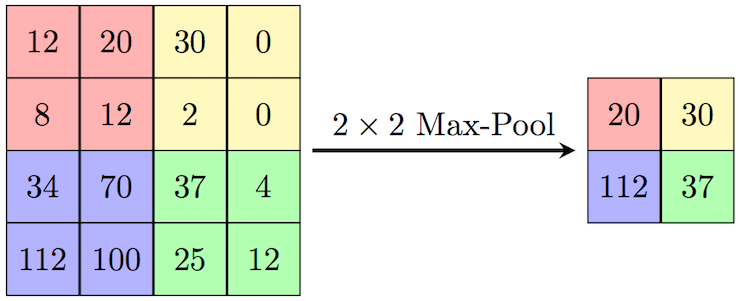
\includegraphics[width=0.75\textwidth]{max_pooling.png}
% where an .eps filename suffix will be0 assumed under latex,
% and a .pdf suffix will be assumed for pdflatex
\caption{ This is an example of max pooling on a 4x4 input with filter size 2x2.   }
\label{fig_max_pool}
\end{figure} 

\subsection{Batch Normalization}
    Convolutional neural networks are difficult to train. 
    The fact that the weights of every layer change every iteration as the deep network learns makes it so that even a small change in the beginning of the network will get amplified as it goes deeper in the network.
    This problem is the internal covariate shift in the network and can be fixed using batch normalization. 
    Batch normalization normalizes each layer in the network for each training batch. 
    Batch normalization is shown in figure ~\ref{fig_batch_norm}. 
    Using batch normalization helps to reduce the problem of the vanishing or exploding gradient and allows for the use of higher learning rates \cite{DBLP:journals/corr/IoffeS15}. 
    This will help models become more stable as well as train faster. 
    The use of batch normalization also helps to regularize the model and prevent overfitting \cite{DBLP:journals/corr/IoffeS15}. 
    Since batch normalization utilizes mini-batches then it will be less useful for batch sizes that are small as the variance in the batches will be greater.

\begin{figure}[tbh]
\centering
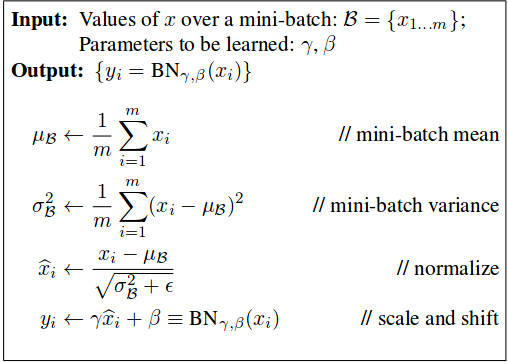
\includegraphics[width=0.5\textwidth]{batch_norm.png}
% where an .eps filename suffix will be0 assumed under latex,
% and a .pdf suffix will be assumed for pdflatex
\caption{ This is how batch normalization would be implemented in the model. The input would be a minibatch and the output would be the input normalized using the mini-batch mean and variance while also scaled and shifted. The batch normalization layers also add parameters for the network to learn, scale and shift. Image is from \cite{DBLP:journals/corr/IoffeS15}. }
\label{fig_batch_norm}
\end{figure} 






\chapter{Methods}
%

\section{Overview of our approach}
We train the most popular models for semantic segmentation for this highly diverse dataset. 
We train and test the networks on 2D slices of the rat brain MRI images. 
The trained networks input is an image slice of the MRI image and the output from the trained network is the segmentation mask. 
We start with 2D slices because it makes the networks much easier to train when compared to a 3D model as well as it uses much less memory. 
Using a 3D model though it is able to learn information along the slice direction as well. 
This information could be useful when learning semantic segmentation as the segmented regions are 3D in real life not 2D. 
Using the 3D volumes though requires a lot more time and memory to train. 
We mainly utilize dice coefficient loss in order to train the model.

\section{Deep Convolutional Neural Network Architecture}
We explore several convolutional neural networks in this thesis, mainly focusing on U-net and dilation networks. 
We choose to implement U-net and dilation networks because they were previously shown to be the most successful for the task of semantic segmentation, each having their own benefits \cite{DBLP:journals/corr/LongSD14}, \cite{DBLP:journals/corr/RonnebergerFB15}, \cite{Yu2016MultiScaleCA}. 
U-net is one of the most popular networks used for medical images and provides excellent results. 
Dilation networks or networks with dilated convolutions also have excellent results for the task of semantic segmentation and is widely used. 

\subsection{U-net}
%
The U-net architecture has been very successful in semantic segmentation. 
U-net works very well because it extends the idea of fully convolutional networks like pooling and convolution layers to upsampling and deconvolutional layers \cite{DBLP:journals/corr/RonnebergerFB15}.
U-net has a base architecture shown in figure ~\ref{fig_Unet}. 
Each black arrow represents a pooling layer when pointing down or an unsampling layer when pointing up. 
The skip connections or concatenation layers are represented by gray arrows between the corresponding layers. 
The filter size is shown as the third dimension in the image size of each block except for the input layer where it corresponds to the image input. 
There is also batch normalization after each convolution layer.
It is made up of four downsampling and four upsamplings layers with two convolutional layers in between. 
The reason that we have the upsampling layers is because we need the output to be a segmentation map of every pixel in the input.
We use deconvolution layers in order to upsample back to the original image size. 
The network also doubles the amount of features every time the network downsamples and halves the number of features every time it upsamples. 
This allows the network to be able to learn more robust contextual information by being able to use more combinations of the features from the previous layer, but also keep the important features as the model upsamples \cite{DBLP:journals/corr/RonnebergerFB15}. 
The input of the architecture is the image size in this case 256x256x3, but can be any image size as long as it is large enough to go through the downsampling layers.
For RGB images usually all three of those slices are put into the model for it to learn but with MRI images they are gray scale images and so only one slice is needed. 
The total amount of parameters in U-net is around 7 million. 
The number of parameters is important because that determines how well a model learns. 
A model with more parameters will take longer to train but will be able to learn more complex connections. 
Too many parameters though is not the best as your model will just learn the training dataset and will not be able to generalize well. 


U-net utilizes downsampling layers to leads to larger receptive field sizes \cite{DBLP:journals/corr/LongSD14}. 
The receptive field size is important because it determines where the network will look and so it is important to ensure that the receptive field size covers the relevant regions \cite{NIPS2016_6203}.
After the image is downsampled it is them upsampled back to its original size for the task it is learning.
In the case of semantic segmentation, the output of the model is required to be the same size as the input so that every pixel can have a probability associated with it.
The reason that U-net is so successful is the skip connections between the downsampled part and upsampled part of the network.
There is a skip connection from one layer of the downsampled network to the corresponding upsampled layer in the network so the first downsampling part is skip connectioned to the last upsampling layer. 
They help to not only preserve the shallow data that was lost in the downsampling, but keep the deep, semantic information to help training significantly \cite{DBLP:journals/corr/LongSD14}.



\begin{figure}[tbh]
\centering
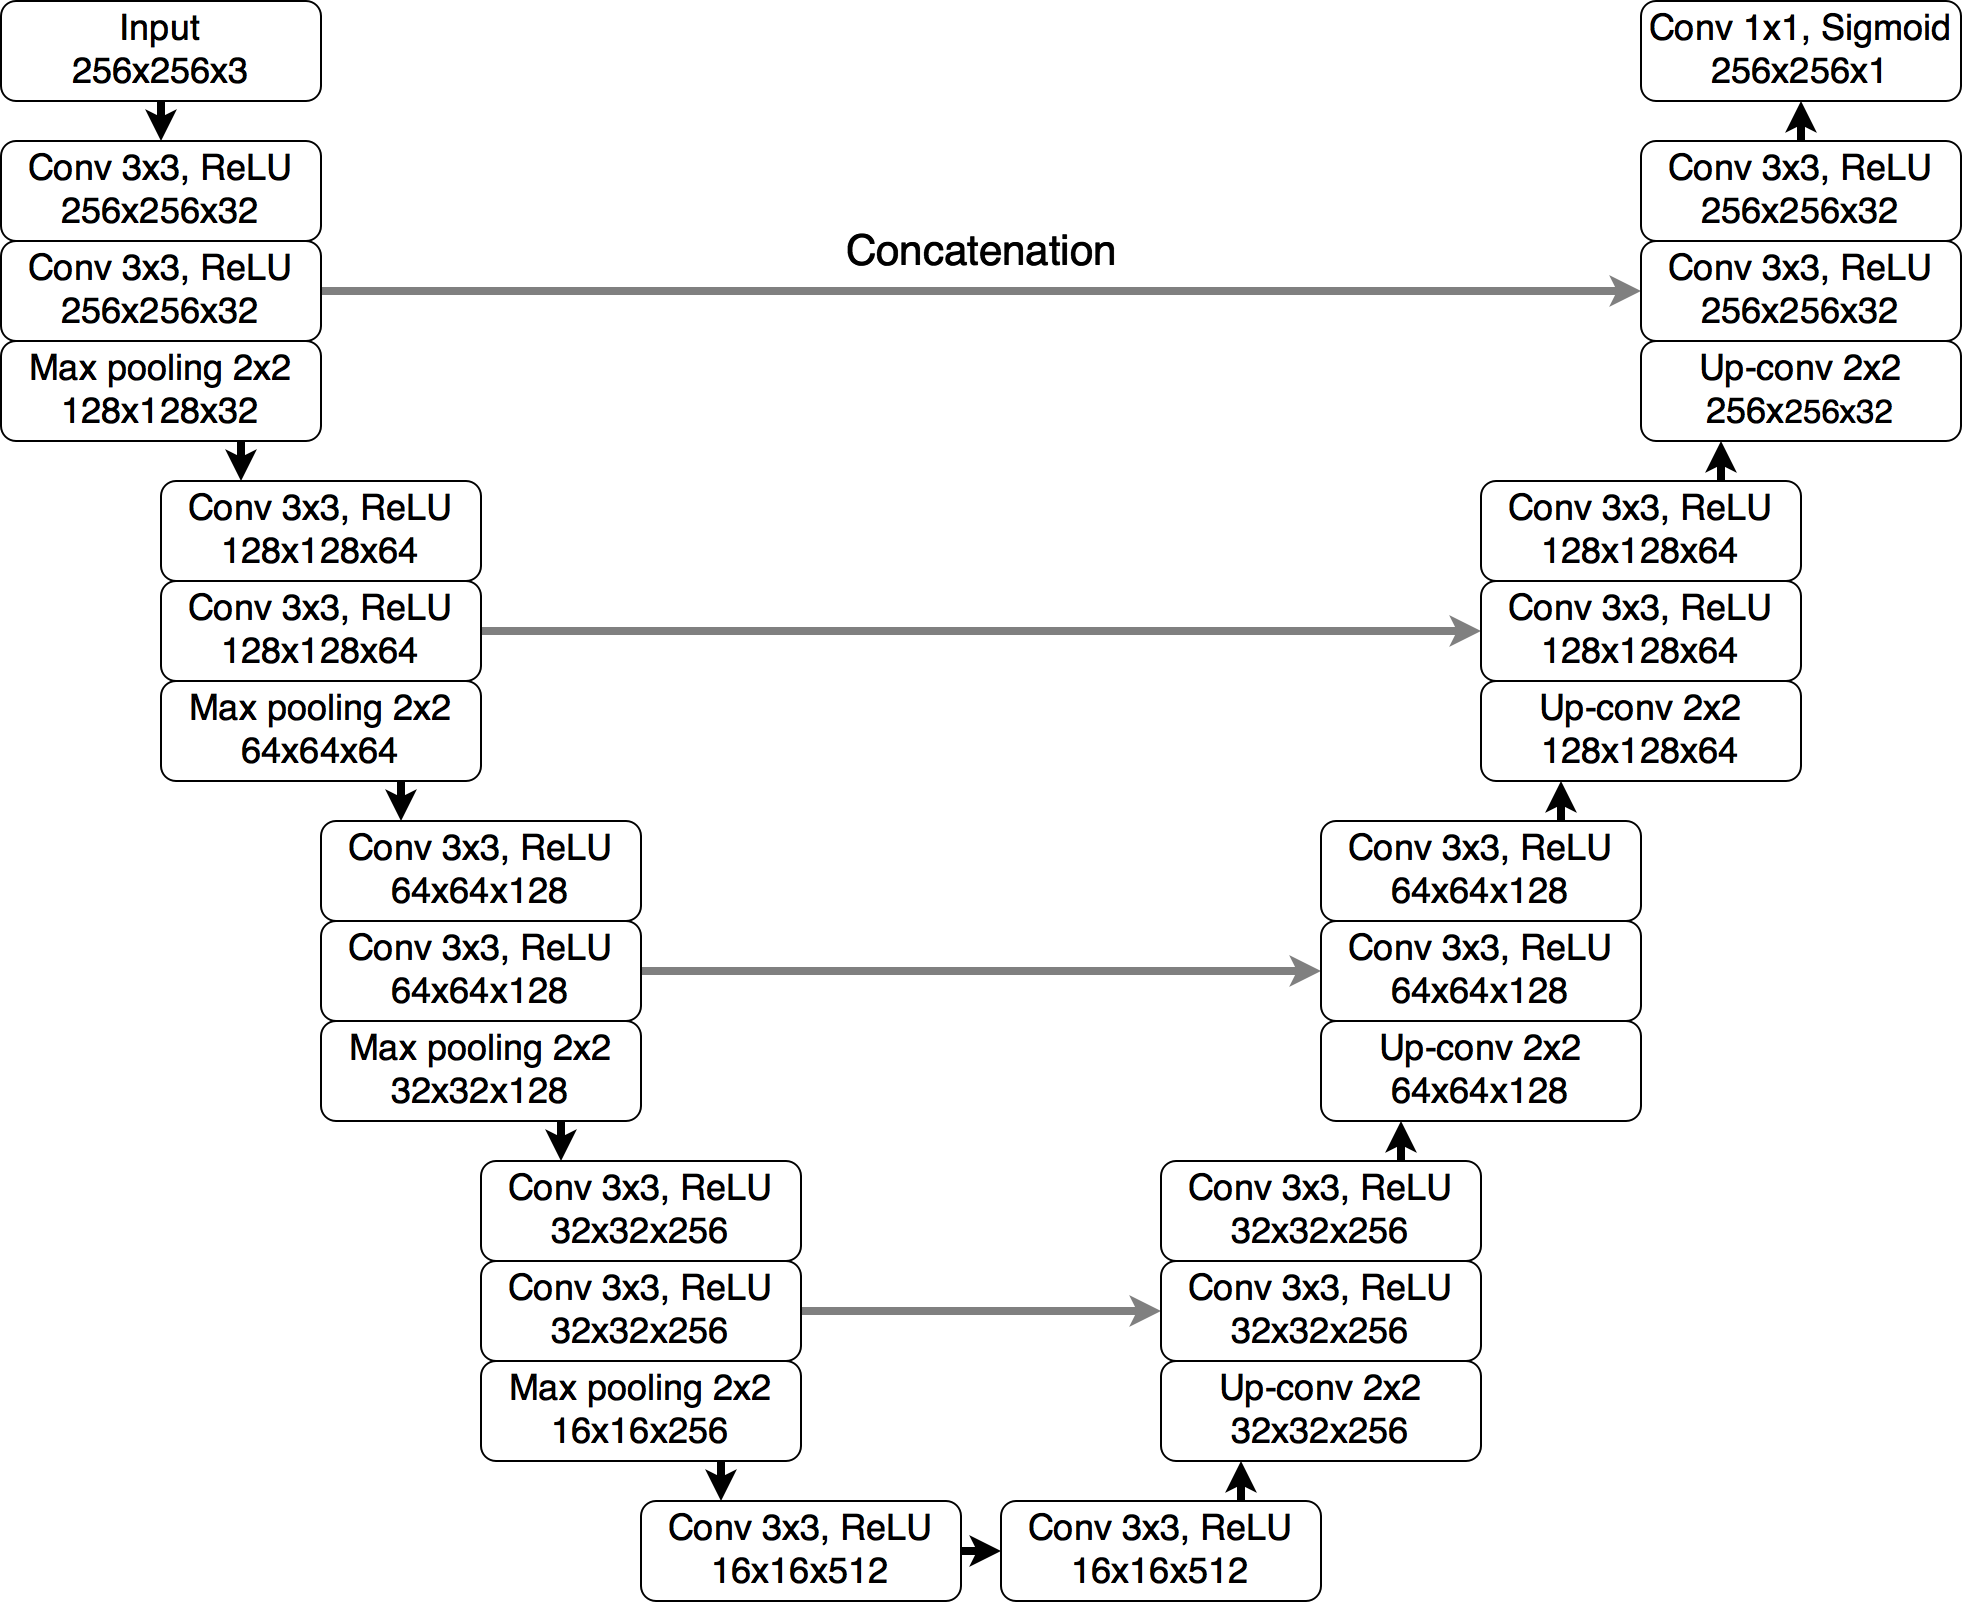
\includegraphics[width=\textwidth]{Unet_Architecture.png}
% where an .eps filename suffix will be assumed under latex,
% and a .pdf suffix will be assumed for pdflatex
\caption{Unet base architecture with input image 256x256x3.}
\label{fig_Unet}
\end{figure}

\subsection{Dilated Convolutions}
Dilated or atrous convolutions are another successful way where semantic segmentation has been implemented. 
Dilated convolutions are utilized because in order for semantic segmentation to be successful, one needs contextual information, as explained before dilated convolutions are really great at contextualizing information using the dilation factors. 
Some of the more popular methods that dilated convolutions are used for is to aggregate multi-scale contextual information  \cite{Yu2016MultiScaleCA}. 
One of the main ways dilated layers do this is with a contextual block. 
This contextual block consists of multiple dilated convolutions in order to get the full context of the input layer. 
An example of the contextual block is shown in figure ~\ref{tab.dilated_context}.
This contextual block is usually put at the end of the network in order to learn the context from the filters created from the previous network. 
The receptive field sizes increase not only as the layers increase, but as the dilation increases as well.
The first two layers have a dilation of 1 or with a dilation factor of 0 so the receptive field size does not increase significantly. 
The layers with dilation though increase the receptive field size significantly until after layer 6 where the receptive field size becomes 65x65. 
We can go further and add a 32 dilation and that would bring our receptive field size to 129x129 if needed. 
This is not needed if the input image is sized below 129x129 as our receptive field size would be larger than the input image creating a lot of unnecessary computation. 
Zero padding is added before every dilated convolution layer in order to keep the same image size throughout the contextual block.

\begin{table}[tbh]
% increase table row spacing, adjust to taste
\renewcommand{\arraystretch}{0.7}
% if using array.sty, it might be a good idea to tweak the value of
% \extrarowheight as needed to properly center the text within the cells
\centering
% Some packages, such as MDW tools, offer better commands for making tables
% than the plain LaTeX2e tabular which is used here.
\begin{tabular}{|c |c|c|c|c|c|c|c|c|}
\hline
\textbf{Layer} & 1 & 2 & 3 & 4 & 5 & 6 & 7 & 8\\
\hline
\hline
Convolution & 3x3 & 3x3 & 3x3 & 3x3 & 3x3 & 3x3 & 3x3 & 3x3\\      
\hline
Dilation & 1 & 1 & 2 & 4 & 8 & 16 & 1 & 1\\
\hline
Truncation & Yes & Yes & Yes & Yes & Yes & Yes & Yes & No\\
\hline
Receptive field & 3x3 & 5x5 & 9x9 & 17x17 & 33x33 & 65x65 & 67x67 & 69x69\\
\hline
\end{tabular}
\caption{Dilated contextual block. It is made up of multiple dilated convolution layers that slowly grow in dilation size to increase the receptive field size to 69x69. Table is from \cite{Yu2016MultiScaleCA}.}
\label{tab.dilated_context}
\end{table}

 
 One of the more popular models that has been adapted for dilated convolutions is VGG16. 
 VGG16 is a very widely used model for classification but has been adapted for many different tasks including semantic segmentation \cite{Simonyan15}. 
 VGG16 model is shown in figure ~\ref{fig_vgg16}. 
 VGG16 is originally used for classification which is why the output of the model is a 1x1x1000. 
 For the task of semantic segmentation though we add zero padding before each layer to preserve the image size so the output is the same size as the input. 
 The first three pooling layers stride is changed to 1 in order to preserve the image size. 
 The last two pooling blocks are also removed and replaced by 3 dilation layers of dilation rate 1. 
 This makes the model simpler and easier for it to learn. 
 The contextual block is then put at the very end with zero padding in between each dilation layer \cite{Yu2016MultiScaleCA}. 
 This model proved to be too large to fit the MR images from this thesis and so in this thesis we modify the VGG model by halving the number of filters used in every layer. 
 The VGG-16 model used in this thesis stacks the halved filter VGG-16 model with the contextual block for the dilated convolutions coming at the end. 
 We will refer to this model as the modified dilation VGG-16 model and is shown in figure ~\ref{fig_modvgg16}.
 As the model decreases the image size stays the same while the filter size increases.
 The total amount of parameters for this model is around 4 million. 
 This is significantly less than U-net. 
 
 \begin{figure}[tbh]
\centering
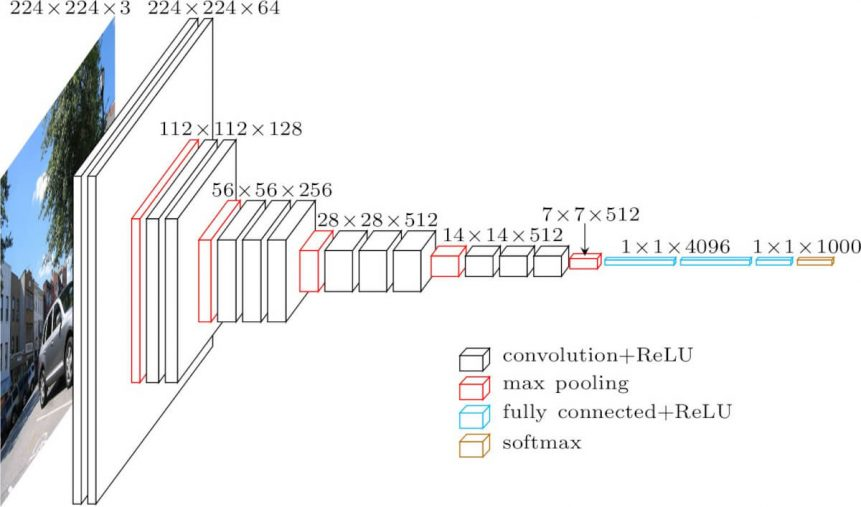
\includegraphics[width=\textwidth]{vgg16-neural-network.jpg}
% where an .eps filename suffix will be assumed under latex,
% and a .pdf suffix will be assumed for pdflatex
\caption{ This is the original VGG16 architecture. Its convolutional and pooling layers make it a very robust model successfully used for classification. Image is from https://neurohive.io/en/popular-networks/vgg16/.}
\label{fig_vgg16}
\end{figure}
 
\begin{figure}[tbh]
\centering
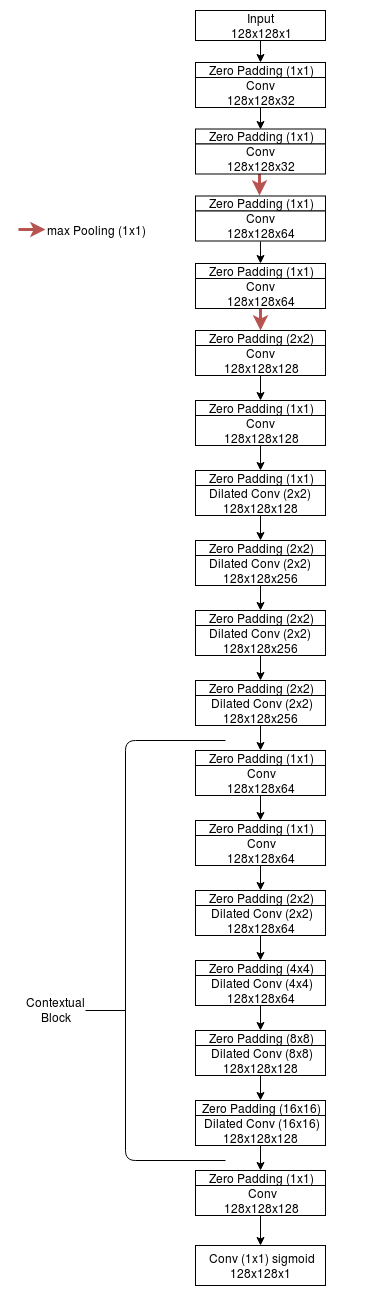
\includegraphics[height=\textheight]{model_VGG16.png}
% where an .eps filename suffix will be assumed under latex,
% and a .pdf suffix will be assumed for pdflatex
\caption{ This is the modified VGG16 architecture. Each Conv layer consists of a 3x3 convolutional kernel. Kernel sizes are mentioned in parenthesis otherwise.}
\label{fig_modvgg16}
\end{figure}
 
\subsection{U-net and dilation network}
Combined U-net with dilated convolutions is a relatively new idea, but has seen preliminary success in the segmentation of medical images \cite{10.1007/978-3-030-01449-0_16dilatedunet}, \cite{DBLP:journals/corr/abs-1805-10720}. 
The success of the U-net dilation networks comes from the idea of using the strength of both U-net and dilated convolutions together. 
The strength of U-net to find the relevant features combined with the strength of dilated convolutions to combine a multitude of features using the larger receptive field sizes. 
This combination can allow the network to learn about features that would previously be lost in pooling. 
The dilation contextual block was usually put at the lowest bottleneck of U-net to ensure that the most relevant features were combined \cite{10.1007/978-3-030-01449-0_16dilatedunet}. 
This is because the smallest bottleneck of U-net or when the downsampling stops is where the most important features for learning are and where we can get the most relevant features combined in many different ways according to the dilation. 
    
We implement this by taking our U-net architecture and applying the dilated contextual block within the bottleneck layer instead of convolutional layers. 
When the dilated contextual block is applied on the bottleneck layer the feature space size is not that large because of all the downsampling layers. 
This helps to preserve space within the model and facilitate training.
In order to fully test this we implement the contextual layer with two to four downsampling layers.
We will refer to this model as the U-net dilation 2-4 downsampling model throughout this thesis and U-net dilation 3 downsampling model is shown in figure ~\ref{fig_modDilUnet}.
The total amount of parameters for the 2-4 downsampling layers are around 9 million, 10 million, and 13 million respectively. 
This is much more compared to U-net which allows the U-net dilation models to learn much more complex connections. 
    
 \begin{figure}[tbh]
\centering
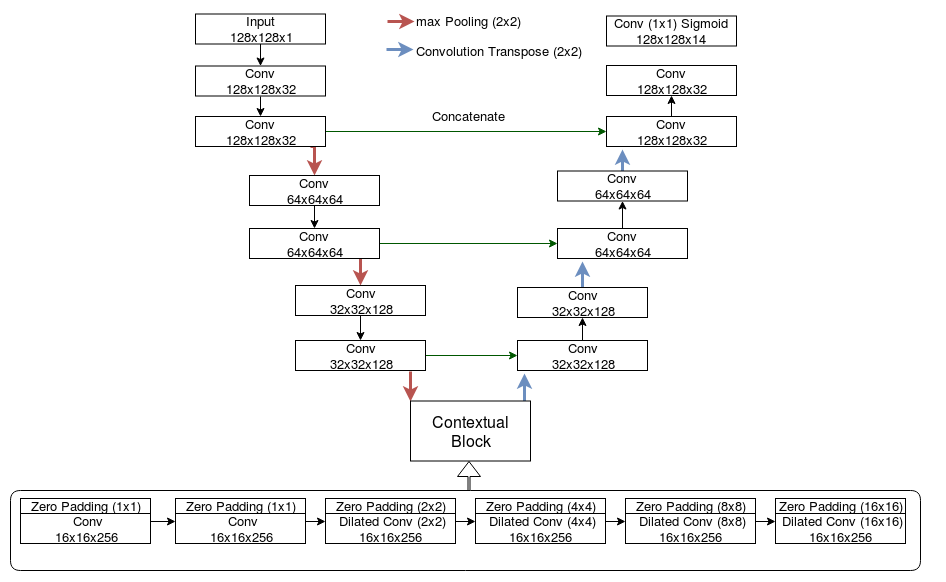
\includegraphics[width=\textwidth]{model_dilunet.png}
% where an .eps filename suffix will be assumed under latex,
% and a .pdf suffix will be assumed for pdflatex
\caption{ Dilation U-net 3 downsampling architecture. The 2 and 4 downsampling dilation U-net models have 2 and 4 downsampling layers correspondingly.}
\label{fig_modDilUnet}
\end{figure}

    
\section{Loss Functions}
    In the task of semantic segmentation there are two loss functions that are mainly used, dice coefficient and cross-entropy. 
    Loss functions are used to let the model know what to optimize for.
    There are pros and cons to both of the loss functions and each had their own fixes for their weaknesses. 
    It is not exactly clear which loss function is the best to use with some papers using cross entropy \cite{DBLP:journals/corr/ChenPK0Y16} and most others using dice coefficient \cite{10.1007/978-3-030-01449-0_16dilatedunet}, \cite{DBLP:journals/corr/abs-1805-10720}. Some of the reasoning to use dice coefficient rather than cross entropy is that dice coefficient directly maximizes the overlap between the segmented region and ground truth, i.e., the accuracy of the segmentation. 
    This thesis is mainly concerned with the accuracy of the segmentation, so we will focus on the dice coefficient.
    
    
\subsection{Dice Coefficient}
    Dice coefficient (DC) was first introduced as a simple spatial overlap measure \cite{10.2307/1932409dice}. 
    Dice coefficient became a very useful measure of spatial overlap which is very helpful in the task of semantic segmentation \cite{dice2004}. 
    Dice Coefficient can be calculated below where A and B are regions that need to be compared
\begin{equation}
 DC = \frac{2*|A \cap B|}{|A| + |B|}\label{eq:dicescore} 
\end{equation}
    $|A|$ and $|B|$ represent the number of elements in each set. 
    If the regions in A and B directly match the the union of the two will give the total number of elements in the region. 
    The denominator will give the total number of elements in A and B which will match the numerator. 
    The max value of the dice score is one and the min value is zero when the union between the two sets is zero. 
    The negation of the calculation of the dice coefficient can be used as a loss function for the model to learn from. 
    Dice coefficent metric performs better with class imbalances because it is a ratio of the predicted and the ground truth. 
    Dice coefficient though is more unstable when training a model because the derivative of this function is not easily calculated and blows up easier.
    
    One problem that arises when trying to train networks using the DC is if there are slices of the volume that do not have ground truths associated for it then we can get a division by zero. 
    This is problematic for training because it is very hard for every region to be segmented to be in every slice in the MRI volume, especially if you want multiple regions segmented. 
    The solution for this is the add a smoothing factor to the DC to prevent dividing by zero. 
    In this case one is added the the numerator and the denominator of the fraction to calculate the DC.
    
    \begin{equation}
 DC = \frac{2*|A \cap B| + 1}{|A| + |B| + 1}\label{eq:dicescoreloss} 
\end{equation}
    By adding one to the numerator and denominator we change the calculation of the DC a bit, but get rid of the division by zero case as well as keep the range of values from [0,1]. 
    This allows for the DC to be used in training a model using backpropagation. 
    

\subsection{Cross-Entropy}
    Cross-entropy (CE) as a loss function has been used widely in training models as it is simple and effective method to train models \cite{deBoer2005}. 
    Cross entropy can be calculated below where $M$ represents the total number of classes, $y_c$ represents the correct classification for $c$, and $p$ represents predicted probability it belongs to class c. 
\begin{equation}
 CE = -\sum_{c=1}^{M}{y_{c}log(p_{c})}  \label{eq:crossentropy} 
\end{equation}
    The min value of cross-entropy is zero where the model is able to predict with full confidence the correct class. 
    Cross-entropy punishes the predictions with the wrong label with high confidence the greatest as it had a higher significance on the loss function. 
    Cross entropy is also clearly defined in backpropogation unlike dice coefficient. 
    Cross-entropy though does not work well for class imbalances as it will give the larger classes priority over the smaller classes.
    This is a big deal for semantic segmentation because a lot of the time the regions that are needed to be segmented are small. 

\chapter{Data}

\section{Description of Data}
    As explained in Chapter 1 the data that will be used is provided by the Center for Molecular Imaging and are MRI rat brain images over time. 
    The MR images themselves vary between each different rat, but also as seen can vary significantly in each group.
\subsection{Brain Regions}
    The brain regions that we will segment are shown in in figure ~\ref{fig:segmentation regions}. 
    There are 7 total regions listed in the image. 
    The only region that is segmented that isn't in the figure is the cerebellum. 
    Each region will also be separated in to a left and a right side region of the brain except for the medial thalamus. 
    This means that in total our model will segment 14 different regions. 
    Each of these regions are very different where we have some that are quite close to each other, the inner and outer cerebral cortex layers, and others that are all alone, the piriform cortex. 
    There are also very small regions like the medial thalamus and very large regions like the cerebellum to take into account. 
    
\begin{figure}
  \centering
  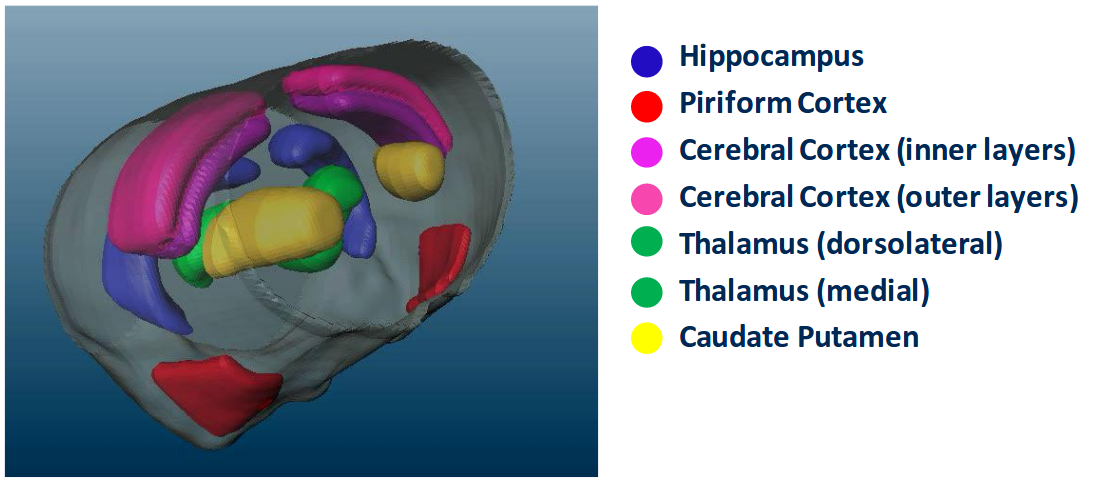
\includegraphics[width=\linewidth]{segmentation_areas.png}
  \caption{MRI rat brain segmentation regions relative to the brain. Image provided by Brad Hobson. }
  \label{fig:segmentation regions}
\end{figure}

    

\subsection{Image Pre-processing}
    Before the rat brain MR images can be used in the model they need to be pre-processed to facilitate training. 
    The rat brain MRI images are taken as nifty files. 
    An example of an unprocessed MR image vs the processed MR image is shown in figure ~\ref{fig:procvsUnproccMRI}.
    The processed image is larger and better contrasted than the pre-processed image, which will help the model train faster.
    We will talk about the exact pre-processing technique as applied to the rat brain MR images.
    
\begin{figure}
\centering
\begin{subfigure}{.5\textwidth}
  \centering
  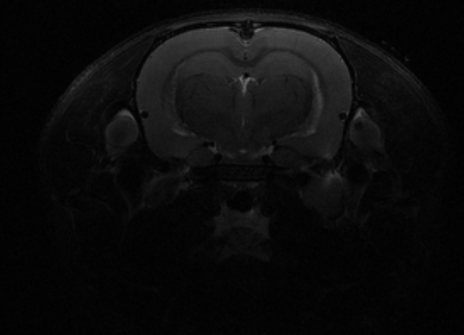
\includegraphics[width=0.9\linewidth]{MRI_veh01.png}
  \caption{Unprocessed T2w MR image }
  \label{fig:unprocessedMRI}
\end{subfigure}%
\begin{subfigure}{.5\textwidth}
  \centering
  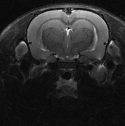
\includegraphics[width=0.8\linewidth]{post_MRI_veh01.png}
  \caption{Pre-processed T2w MR image}
  \label{fig:processedMRI}
\end{subfigure}
\caption{This figure shows the image pre-processing technique as applied to the rat brain MR images.}
\label{fig:procvsUnproccMRI}
\end{figure}

\subsubsection{Normalization and Cropping}
    One of the first things we do to the image is center cropping. 
    As shown in the unprocessed MRI image the rat brain is covered with a lot of background pixels unneeded for the model.
    In order to make the model more efficient the images are center cropped and downsampled from 280x200x44 to 128x128x44.
    This helps to emphasize the more important regions and leave out the areas that are not useful for the model. 
    We also downsample the images to 128x128 in order to be able to have enough space in the gpu to be able to train the model.
    
    The images are then normalized in order to keep the range of the images the same and decrease the bias in the model. 
    They are normalized by dividing by the max pixel value per MRI volume or 128x128x44 image.


\subsubsection{Biased MRI images}
     One very important processing technique used for MR images is that they need to be corrected for the bias field signal. 
     This signal is produced when taking the MRI images and causes a fluctuation in the gray values in the MRI image. 
     This can be corrected for by estimating the bias field signal using a surface fitting approach \cite{Juntu2005BiasFC}. 
     As seen in figure ~\ref{fig:biasedvscorrMRI}, the fluctuations caused by the bias signal can be very large and greatly affect the performance of the model. 
    
\begin{figure}
\centering
\begin{subfigure}{.5\textwidth}
  \centering
  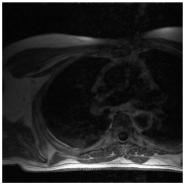
\includegraphics[width=.6\linewidth]{baisedMRIimage.png}
  \caption{Example of a biased MRI image due to the bias field signal}
  \label{fig:baisedMRI}
\end{subfigure}%
\begin{subfigure}{.5\textwidth}
  \centering
  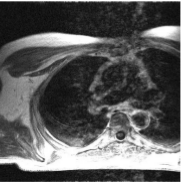
\includegraphics[width=.6\linewidth]{CorrectedMRIBias.png}
  \caption{The same image but corrected for the bias field signal using the surface fitting approach}
  \label{fig:correctedMRI}
\end{subfigure}
\caption{This figure shows some the effect of bias field signal on MRI images. }
\label{fig:biasedvscorrMRI}
\end{figure}
    

\subsection{Data Augmentation}
    Data augmentation is very useful in machine learning tasks. 
    One of the main ways to have a model generalize better is to train the model on a more diverse dataset. 
    Data Augmentation takes advantage of basic image transforms to "create" new images for the model to train on \cite{articledataAug}. 
    Some examples of basic data augmentation transforms are scale, crop, brightness, rotation, flipping, padding, etc. 
    All of these basic transforms when applied to an image will change the image and when put through the model will allow it to be more robust. 
    Many papers utilize data augmentation in order to increase the robustness and precision of their model ~\cite{NIPS2012_Krizhevsky}, ~\cite{articledataAug}, ~\cite{DBLP:journals/corr/MilletariNA16}, ~\cite{DBLP:journals/corr/RonnebergerFB15}.
    Other papers though report that data augmentation didn't improve their results significantly or didn't use data augmentation ~\cite{DBLP:journals/corr/HavaeiDWBCBPJL15}, ~\cite{DBLP:journals/corr/abs-1805-10720}. 
    When it comes to data augmentation for medical images, the methods that do utilize data augmentation only use a certain amount of transformations ~\cite{10.1007/978-3-030-01449-0_16dilatedunet}. 
    The reason behind this is that medical images are usually taken in a controlled environment where the patient is made to lay in a bed and not move as much as they can. 
    For this reason, in this paper we only adopt a rotation of 10 degrees, horizontal flip, image shift of 20\%, and a brightness range from 70\% to 100\%.
    We implement a small rotation as well as well as a small image shift and horizontal flip because not all images are taken perfectly in the same area every time even though it is a controlled environment. 
    A brightness range is also implemented because depending on the injected dose the tissue will be brighter or darker compared to the surrounding tissue. 
    Some examples of the data augmented images are shown in figure ~\ref{fig:dataAugImage}. 
    

\begin{figure}[ht] 
  \begin{minipage}[b]{0.5\linewidth}
    \centering
    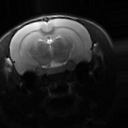
\includegraphics[width=\linewidth]{0.png} 
  \end{minipage} 
  \begin{minipage}[b]{0.5\linewidth}
    \centering
    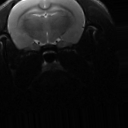
\includegraphics[width=\linewidth]{1.png} 
  \end{minipage} 
  \begin{minipage}[b]{0.5\linewidth}
    \centering
    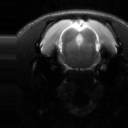
\includegraphics[width=\linewidth]{3.png} 
  \end{minipage}
  \hfill
  \begin{minipage}[b]{0.5\linewidth}
    \centering
    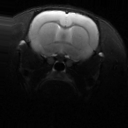
\includegraphics[width=\linewidth]{9.png} 
  \end{minipage} 
  \caption{Some examples of the data augmented MRI images. }
  \label{fig:dataAugImage} 
\end{figure}
\chapter{Experimental results}
    This chapter will discuss the experimental setting used and the results of the trained models.
\section{Experimental Setting}
    The model as well as the hyperparamters are defined using Tensorflow and Keras. 
    The model was trained for single region segmentation as well as multi-region segmentation where all 14 regions were predicted all at once.
    The hyperparemeter set up was slightly different for training a model for a single region vs multiple regions. 
    For the single region training the learning rate was 1e-5 and the batch size was 32 for U-net and 3 for the dilation models. 
    The batch size varied depending on the model as the dilation models needed more memory.  
    The models in the single region were trained for at least 128 epochs in order to ensure that the model was trained sufficiently, but not over fitting the data. 
    
    For multiple region training the learning used was 2e-5 and the batch size was 32 for U-net and the U-net dilation and 16 for the modified dilation VGG-16 models. 
    The learning rate is larger because since there was much more to learn the models struggled in the beginning to learn well.
    The multiple region models were trained for much longer than the single region training and needed to be trained for at least 300 epochs in order to train the model sufficiently.
    The multiple region models learning rate was changed because the training for those models were much slower and so utilizing a higher learning rate make the learning much faster.
    Each model is trained using the ADAM optimizer as described in ~\cite{Kingma2014AdamAM}. 
    The input images were also shuffled randomly in order to decrease the bias that the model might learn. 
    The experiments were trained on a 10GB NVIDIA GTX 1080 Ti. 
    
\subsection{Image Data}
    As explained before a total of 40 rats were imaged with a total of 120 MRI images taken. 
    Due to some problems with imaging only 115 animal scans were available for use within the model. 
    The data was split between a training set, a validation set, and test set. 
    Since the data is also split between 4 different animal groups the validation and test dataset has one animal from each group to see how each group performs from the model. 
   Each animal has MR images at three different time points as well and so the validation/test sets consist of 12 different animal MR images while the training dataset consists of 103 animal MR images. 
    Data augmentation was also utilized as explained before and the dataset was doubled and data augmentation applied to the replicated data. 
    The training dataset consists of a total of 206 MR images each of size 128x128x44 or 9,064 total 2D 1MR images while the validation and test sets consists of 12 MR images each of size 128x128xx44 or 528 2D MR images. 

\section{Visualization of segmentation results for single region}
    For the single segmentation, the segmentation chosen was for the medial thalamus. 
    This region was chosen because it was the smallest region as well as a region that changed throughout the groups.
    

\subsection{Models}
    This section is dedicated to show the different models tested and to compare them for single region segmentation of the MR images. 
    This is very challenging because the regions are so small within the 128x128x44 MRI images that the model needs to take that into account. 
    Table `\ref{tab.single_model_results} shows the results for the average dice score coefficient for single region segmentation.
    U-net gave the most consistent answers and was the easiest to implement while there were some problems when training the dilation VGG-16 model.
    U-net performs much better than dilation VGG-16 in the training data but not much better according to the validation data and we see they are quite close with u-net only slightly outperforming dilation VGG-16. 
    Let us take a closer look at each model.
    
\begin{table}[tbh]
% increase table row spacing, adjust to taste
\renewcommand{\arraystretch}{1}
% if using array.sty, it might be a good idea to tweak the value of
% \extrarowheight as needed to properly center the text within the cells
\centering
% Some packages, such as MDW tools, offer better commands for making tables
% than the plain LaTeX2e tabular which is used here.
\begin{tabular}{|c|c|c|}
\hline
\textbf{Model} & \textbf{training DSC} & \textbf{validation DSC}\\
\hline
U-net & 0.997 & 0.811\\ %weights_singleLabel1_dilation_2_300.h5     
%#\hline
%dilation layer & 0.0000\\%weights_singleLabel1_reduceModel_1_128.h5
\hline
dilation VGG-16 & 0.698 & 0.801\\ %weights_singleLabel1_1_128.h5 
\hline
\end{tabular}
\caption{DSC scores comparing U-net and the dilation VGG-16 models}
\label{tab.single_model_results}
\end{table}


\subsubsection{U-net}
    Here are the training results for single region u-net as discussed before. 
    Figure ~\ref{fig:results_single_unet_train} shows the training and validation results of the model. 
    U-net was able to learn the training dataset very well with a training DSC of 0.99 while the validation dataset leaned quite well at 0.803.
    After the 50 epoch the model DSC didn't go up much at all and stabilized while the training DSC slowly increased.
    Table ~\ref{tab.single_model_results_Unet} shows the overall results for the model. 
    The control group or VEH results aren't available for this calculation.
    What is interesting is that the model performs the best on the D28 images for DFP and MDZ. 
    The D28 images especially for DFP are the most inconsistent because of brain cell death from seizures, while the D03 images are the most consistent as they are the closest to a healthy rat brain. 
    This is also shown in the variation among the DSC of the D03 data compared to the D28 data, where the D03 data is more consistent than the D28 data. 
    
    
\begin{figure}[tbh]
\centering
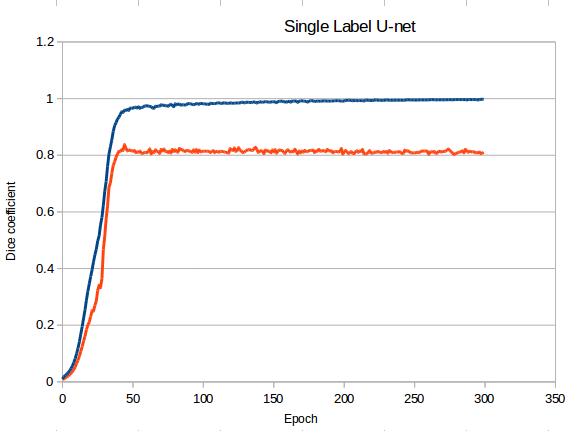
\includegraphics[width=\textwidth]{results/train_results_single_unet.png}
% where an .eps filename suffix will be assumed under latex,
% and a .pdf suffix will be assumed for pdflatex
\caption{Training the U-net model. Blue curve is training curve and the red curve is the validation curve. }
\label{fig:results_single_unet_train}
\end{figure}

\begin{table}[tbh]
% increase table row spacing, adjust to taste
\renewcommand{\arraystretch}{1}
% if using array.sty, it might be a good idea to tweak the value of
% \extrarowheight as needed to properly center the text within the cells
\centering
% Some packages, such as MDW tools, offer better commands for making tables
% than the plain LaTeX2e tabular which is used here.
\begin{tabular}{|c|c|c|c|}
\hline
\textbf{Group} & \textbf{D03}& \textbf{D07}& \textbf{D28}\\
\hline
DFP & 0.755 & 0.836 & 0.872\\      
\hline
DZP & 0.765 & 0.814 & 0.788\\
\hline
MDZ & 0.821 & 0.769 & 0.832\\ 
\hline
\end{tabular}
\caption{DSC scores of test data for single model U-net}
\label{tab.single_model_results_Unet}
\end{table}


    Figure ~\ref{fig:results_single_unet_DFP} shows the results when applied to the DFP test images. 
    If we compare the different days the biggest difference are the D28 images compared to the D03 and D07 images. 
    The medial thalamus shifted as brain changed due to the seizures. 
    The brighter regions or the ventricles also increased significantly compared to in the beginning. 
    When just looking at the results it seems they match up quite well with the ground truth with some minor differences. 
    Figure ~\ref{fig:results_single_unet_DZP} and figure ~\ref{fig:results_single_unet_MDZ} show the results for the DZP and the MDZ test images, relatively.
    If we compare the DZP and MDZ images with the DFP images the ventricles in the DZP and MDZ are much smaller and the general shape of the brain hasn't changed as significantly as the DFP animals.
    One interesting thing to note is that in figure ~\ref{fig:results_single_unet_MDZ} the day 28 image has a ground truth but no prediction. 
    This is interesting because it shows that the model has to learn to segment the regions that are on different slice numbers or grouped with different regions. 
    This is were the convolutional layers come into play as they make the model spatially invariant and so no matter which slice the region is at as long as the characteristics are consistent the model will still predict a region. 
    Upon further inspection D28 slice 23 in the MDZ animals is the start of the medial thalamus and in the images where the medial thalamus starts with a very small region like in the MDZ animal case we don't get a prediction. 
    Overall the U-net preforms quite well on the single region segmentation with only some slight differences in the predictions. 
    We will explain later why these slight differences are acceptable. 
    

\begin{figure}[!ht]  
   \centering % <-- added
\begin{subfigure}{0.35\textwidth}
  \includegraphics[width=\linewidth]{results/single_unet/"DFP01 R14-189-D03_23".png}
  \caption{D03 slice 23}
\end{subfigure}\hfil % <-- added
\begin{subfigure}{0.35\textwidth}
  \includegraphics[width=\linewidth]{results/single_unet/"DFP01 R14-189-D03_25".png}
  \caption{D03 slice 25}
\end{subfigure}

\medskip
\begin{subfigure}{0.35\textwidth}
  \includegraphics[width=\linewidth]{results/single_unet/"DFP01 R14-189-D07_23".png}
  \caption{D07 slice 23}
\end{subfigure}\hfil % <-- added
\begin{subfigure}{0.35\textwidth}
  \includegraphics[width=\linewidth]{results/single_unet/"DFP01 R14-189-D07_25".png}
  \caption{D07 slice 25}
\end{subfigure}

\medskip
\begin{subfigure}{0.35\textwidth}
  \includegraphics[width=\linewidth]{results/single_unet/"DFP01 R14-189-D28_23".png}
  \caption{D28 slice 23}
\end{subfigure}\hfil % <-- added
\begin{subfigure}{0.35\textwidth}
  \includegraphics[width=\linewidth]{results/single_unet/"DFP01 R14-189-D28_25".png}
  \caption{D28 slice 25}
\end{subfigure}
  
  \caption{Results for DFP animal group at day 3, day 7, day 28 on single region U-net. The red region is the predicted output the model sent and the blue region is the ground truth.}
  \label{fig:results_single_unet_DFP}
\end{figure}


\begin{figure}[!htb]  
\centering % <-- added
\begin{subfigure}{0.35\textwidth}
  \includegraphics[width=\linewidth]{results/single_unet/"DZP01 R14-187-D03_23".png}
  \caption{D03 slice 23}
\end{subfigure}\hfil
\begin{subfigure}{0.35\textwidth}
  \includegraphics[width=\linewidth]{results/single_unet/"DZP01 R14-187-D03_25".png}
  \caption{D03 slice 25}
\end{subfigure}

\medskip
\begin{subfigure}{0.35\textwidth}
  \includegraphics[width=\linewidth]{results/single_unet/"DZP01 R14-187-D07_23".png}
  \caption{D07 slice 23}
\end{subfigure}\hfil
\begin{subfigure}{0.35\textwidth}
  \includegraphics[width=\linewidth]{results/single_unet/"DZP01 R14-187-D07_25".png}
  \caption{D07 slice 25}
\end{subfigure}

\medskip
\begin{subfigure}{0.35\textwidth}
  \includegraphics[width=\linewidth]{results/single_unet/"DZP01 R14-187-D28_23".png}
  \caption{D28 slice 23}
\end{subfigure}\hfil
\begin{subfigure}{0.35\textwidth}
  \includegraphics[width=\linewidth]{results/single_unet/"DZP01 R14-187-D28_25".png}
  \caption{D28 slice 25}
\end{subfigure}
  
  \caption{Results for DZP animal group at day 3, day 7, day 28 on single region U-net. The red region is the predicted output the model sent and the blue region is the ground truth.}
  \label{fig:results_single_unet_DZP}
\end{figure}



\begin{figure}[!htb]  
   \centering % <-- added
\begin{subfigure}{0.35\textwidth}
  \includegraphics[width=\linewidth]{results/single_unet/"MDZ01 R14-190-D03_23".png}
  \caption{D03 slice 23}
\end{subfigure}\hfil % <-- added
\begin{subfigure}{0.35\textwidth}
  \includegraphics[width=\linewidth]{results/single_unet/"MDZ01 R14-190-D03_25".png}
  \caption{D03 slice 25}
\end{subfigure}

\medskip
\begin{subfigure}{0.35\textwidth}
  \includegraphics[width=\linewidth]{results/single_unet/"MDZ01 R14-190-D07_23".png}
  \caption{D07 slice 23}
\end{subfigure}\hfil % <-- added
\begin{subfigure}{0.35\textwidth}
  \includegraphics[width=\linewidth]{results/single_unet/"MDZ01 R14-190-D07_25".png}
  \caption{D07 slice 25}
\end{subfigure}

\medskip
\begin{subfigure}{0.35\textwidth}
  \includegraphics[width=\linewidth]{results/single_unet/"MDZ01 R14-190-D28_23".png}
  \caption{D28 slice 23}
\end{subfigure}\hfil % <-- added
\begin{subfigure}{0.35\textwidth}
  \includegraphics[width=\linewidth]{results/single_unet/"MDZ01 R14-190-D28_25".png}
  \caption{D28 slice 25}
\end{subfigure}
  
  \caption{Results for MDZ animal group at day 3, day 7, day 28 on single region U-net. The red region is the predicted output the model sent and the blue region is the ground truth. }
  \label{fig:results_single_unet_MDZ}
\end{figure}

\subsubsection{Dilation VGG-16}
    Here are the training results for the modified dilation VGG-16 model. 
    Figure ~\ref{fig:results_single_dilation_train} shows the training and validation results. 
    It is interesting to note how the validation DSC is larger than the training DSC.
    This can be attributed to the fact that the validation data is less complex than the training data due to the data augmentation. 
    The dilation VGG-16 model also has much less parameters than U-net and so the model can't learn the more complex training data as well as the validation data. 
    Another interesting thing to note is that the training and validation curves shoot up from the 1st epoch and mainly stabilize at the epoch 20. 
    Table ~\ref{tab.single_model_results_dilation} shows the results of the dilation VGG-16 model on the test data. Compared to U-net the DSC values are much lower for the dilation VGG-16 model. 
    This means that the dilation VGG-16 model doesn't generalize as well as the U-net model. 
    This could be attributed to the parameters of the model or how its structured is not ideal for the single segmentation task. 
    The D03 DSC's in the table are on average a higher DSC compared to D07 and D28 and the variation is smaller. 
    D28 DSC's the average is the least and variation the largest.
    This is because D28 has the most variation so the dilation VGG-16 model became slightly biased to segment the earlier times better since they are more consistent.
    In the case of U-net, it had enough parameters to still be able to learn the D28 dataset as well. 

\begin{figure}[!tbh]
\centering
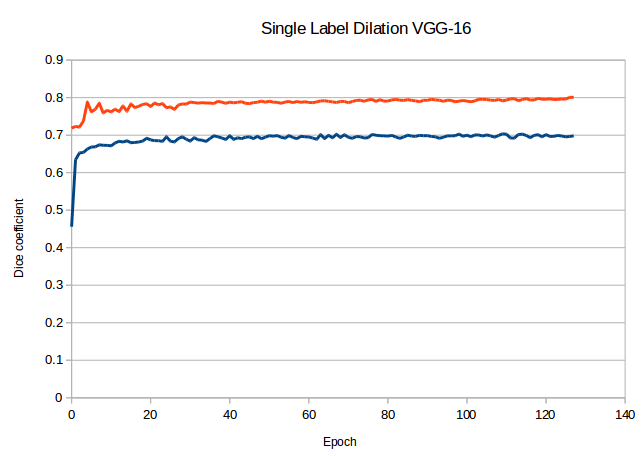
\includegraphics[width=\textwidth]{results/train_results_single_dilation.png}
% where an .eps filename suffix will be assumed under latex,
% and a .pdf suffix will be assumed for pdflatex
\caption{Training the dilation VGG-16 model. Blue curve is training curve and the red curve is the validation curve. }
\label{fig:results_single_dilation_train}
\end{figure}

\begin{table}[tbh]
% increase table row spacing, adjust to taste
\renewcommand{\arraystretch}{1}
% if using array.sty, it might be a good idea to tweak the value of
% \extrarowheight as needed to properly center the text within the cells
\centering
% Some packages, such as MDW tools, offer better commands for making tables
% than the plain LaTeX2e tabular which is used here.
\begin{tabular}{|c|c|c|c|}
\hline
\textbf{Group} & \textbf{D03}& \textbf{D07}& \textbf{D28}\\
\hline
DFP & 0.711 & 0.551 & 0.706\\      
\hline
DZP & 0.729 & 0.681 & 0.563\\
\hline
MDZ & 0.665 & 0.650 & 0.617\\ 
\hline
VEH & 0.649 & 0.675 & 0.635\\ 
\hline
\end{tabular}
\caption{DSC scores of test data for single model dilation VGG-16}
\label{tab.single_model_results_dilation}
\end{table}


Figure ~\ref{fig:results_single_dilation_DFP}, ~\ref{fig:results_single_dilation_DZP}, ~\ref{fig:results_single_dilation_MDZ}, and ~\ref{fig:results_single_dilation_VEH} show the segmentation images of the dilation VGG-16 model applied to the test image. 
Compared to the U-net results the dilation VGG-16 predictions are more circular. 
This causes the regions to match horizontally, but vertically the prediction overshoots the ground truth and lowers the overall DSC.
This is the reason why the DSC for the dilation VGG-16 model performs much lower than U-net.
One difference is that for figure ~\ref{fig:results_single_dilation_MDZ}, MDZ D28 slice 23 the dilation VGG-16 model was able to predict a region though larger than the ground truth where U-net didn't predict a region here. 
Another interesting thing to note is in figure ~\ref{fig:results_single_dilation_DZP} in D28 slice 23 that dilation VGG-16 model predicted the medial thalamus even though there is no ground truth.
This could be attributed to the modified dilation VGG-16 model not learning about the results as well as u-net.
In figure ~\ref{fig:results_single_dilation_DFP} the D07 segmentation got the worst results at a DSC of 0.55 and in slice 23 their is no prediction. 
This is interesting as it seems like the predictions for D07 and D28 are very similar, which causes a better performance for D28 and a worse one for D07.

\begin{figure}[!htb]  
    \centering % <-- added
\begin{subfigure}{0.35\textwidth}
  \includegraphics[width=\linewidth]{results/single_dilation/"DFP01 R14-189-D03_23".png}
  \caption{D03 slice 23}
\end{subfigure}\hfil % <-- added
\begin{subfigure}{0.35\textwidth}
  \includegraphics[width=\linewidth]{results/single_dilation/"DFP01 R14-189-D03_25".png}
  \caption{D03 slice 25}
\end{subfigure}

\medskip
\begin{subfigure}{0.35\textwidth}
  \includegraphics[width=\linewidth]{results/single_dilation/"DFP01 R14-189-D07_23".png}
  \caption{D07 slice 23}
\end{subfigure}\hfil % <-- added
\begin{subfigure}{0.35\textwidth}
  \includegraphics[width=\linewidth]{results/single_dilation/"DFP01 R14-189-D07_25".png}
  \caption{D07 slice 25}
\end{subfigure}

\medskip
\begin{subfigure}{0.35\textwidth}
  \includegraphics[width=\linewidth]{results/single_dilation/"DFP01 R14-189-D28_23".png}
  \caption{D28 slice 23}
\end{subfigure}\hfil % <-- added
\begin{subfigure}{0.35\textwidth}
  \includegraphics[width=\linewidth]{results/single_dilation/"DFP01 R14-189-D28_25".png}
  \caption{D28 slice 25}
\end{subfigure}
  
  \caption{Results for DFP animal group at day 3, day 7, day 28 on single region dilation VGG-16. The red region is the predicted output the model sent and the blue region is the ground truth.}
  \label{fig:results_single_dilation_DFP}
\end{figure}


\begin{figure}[!htb]  
    \centering % <-- added

\begin{subfigure}{0.35\textwidth}
  \includegraphics[width=\linewidth]{results/single_dilation/"DZP01 R14-187-D03_23".png}
  \caption{D03 slice 23}
\end{subfigure}\hfil
\begin{subfigure}{0.35\textwidth}
  \includegraphics[width=\linewidth]{results/single_dilation/"DZP01 R14-187-D03_25".png}
  \caption{D03 slice 25}
\end{subfigure}

\medskip
\begin{subfigure}{0.35\textwidth}
  \includegraphics[width=\linewidth]{results/single_dilation/"DZP01 R14-187-D07_23".png}
  \caption{D07 slice 23}
\end{subfigure}\hfil
\begin{subfigure}{0.35\textwidth}
  \includegraphics[width=\linewidth]{results/single_dilation/"DZP01 R14-187-D07_25".png}
  \caption{D07 slice 25}
\end{subfigure}

\medskip
\begin{subfigure}{0.35\textwidth}
  \includegraphics[width=\linewidth]{results/single_dilation/"DZP01 R14-187-D28_23".png}
  \caption{D28 slice 23}
\end{subfigure}\hfil
\begin{subfigure}{0.35\textwidth}
  \includegraphics[width=\linewidth]{results/single_dilation/"DZP01 R14-187-D28_25".png}
  \caption{D28 slice 25}
\end{subfigure}
  
  \caption{Results for DZP animal group at day 3, day 7, day 28 on single region dilation VGG-16. The red region is the predicted output the model sent and the blue region is the ground truth.}
  \label{fig:results_single_dilation_DZP}
\end{figure}



\begin{figure}[!htb]  
    \centering % <-- added
\begin{subfigure}{0.35\textwidth}
  \includegraphics[width=\linewidth]{results/single_dilation/"MDZ01 R14-190-D03_23".png}
  \caption{D03 slice 23}
\end{subfigure}\hfil % <-- added
\begin{subfigure}{0.35\textwidth}
  \includegraphics[width=\linewidth]{results/single_dilation/"MDZ01 R14-190-D03_25".png}
  \caption{D03 slice 25}
\end{subfigure}

\medskip
\begin{subfigure}{0.35\textwidth}
  \includegraphics[width=\linewidth]{results/single_dilation/"MDZ01 R14-190-D07_23".png}
  \caption{D07 slice 23}
\end{subfigure}\hfil % <-- added
\begin{subfigure}{0.35\textwidth}
  \includegraphics[width=\linewidth]{results/single_dilation/"MDZ01 R14-190-D07_25".png}
  \caption{D07 slice 25}
\end{subfigure}

\medskip
\begin{subfigure}{0.35\textwidth}
  \includegraphics[width=\linewidth]{results/single_dilation/"MDZ01 R14-190-D28_23".png}
  \caption{D28 slice 23}
\end{subfigure}\hfil % <-- added
\begin{subfigure}{0.35\textwidth}
  \includegraphics[width=\linewidth]{results/single_dilation/"MDZ01 R14-190-D28_25".png}
  \caption{D28 slice 25}
\end{subfigure}
  
  \caption{Results for MDZ animal group at day 3, day 7, day 28 on single region dilation VGG-16. The red region is the predicted output the model sent and the blue region is the ground truth. }
  \label{fig:results_single_dilation_MDZ}
\end{figure}


\begin{figure}[!htb]  
    \centering % <-- added
\begin{subfigure}{0.35\textwidth}
  \includegraphics[width=\linewidth]{results/single_dilation/"Veh01 R14-192-D03_23".png}
  \caption{D03 slice 23}
\end{subfigure}\hfil % <-- added
\begin{subfigure}{0.35\textwidth}
  \includegraphics[width=\linewidth]{results/single_dilation/"Veh01 R14-192-D03_25".png}
  \caption{D03 slice 25}
\end{subfigure}

\medskip
\begin{subfigure}{0.35\textwidth}
  \includegraphics[width=\linewidth]{results/single_dilation/"Veh01 R14-192-D07_23".png}
  \caption{D07 slice 23}
\end{subfigure}\hfil % <-- added
\begin{subfigure}{0.35\textwidth}
  \includegraphics[width=\linewidth]{results/single_dilation/"Veh01 R14-192-D07_25".png}
  \caption{D07 slice 25}
\end{subfigure}

\medskip
\begin{subfigure}{0.35\textwidth}
  \includegraphics[width=\linewidth]{results/single_dilation/"Veh01 R14-192-D28_23".png}
  \caption{D28 slice 23}
\end{subfigure}\hfil % <-- added
\begin{subfigure}{0.35\textwidth}
  \includegraphics[width=\linewidth]{results/single_dilation/"Veh01 R14-192-D28_25".png}
  \caption{D28 slice 25}
\end{subfigure}
  
  \caption{Results for VEH animal group at day 3, day 7, day 28 on single region dilation VGG-16. The red region is the predicted output the model sent and the blue region is the ground truth. }
  \label{fig:results_single_dilation_VEH}
\end{figure}


\section{Visualization of segmentation results for multiple regions}
In the following section we now test multi-segmentation for the models described in Chapter 3. 
We will train the models on all 14 different classes and assign them each a different color in the prediction.
The cerebellum is darker blue, hippocampus is sky blue and purple corresponding to right and left sides, dorsolateral thalamus is green and orange corresponding to right and left sides, medial thalamus is yellow, outer cerebral cortex is pink and light purple corresponding to right and left sides, inner cerebral cortex is light blue and black corresponding to right and left sides, caudate putamen is purple and darker blue corresponding to right and left sides, and finally the piriform cortex is green and light orange corresponding to right and left sides.
We train the model using the parameters described above in the experimental settings.



\subsection{Models}
This section is dedicated to comparing and contrasting the different models described in chapter 3.
Table ~\ref{tab.multi_model_results} shows the training results for the different models. 
According to these results U-net trains the best while the dilation VGG-16 trains the worst.
The gap between the training DSC and the validation DSC though is very large for U-net which tells us that the model doesn't generalize as well. 
When we combine the U-net with the dilation contextual blocks then the validation data is much closer to the training data, but the values themselves are low. 
Just comparing the U-net dilation models in the table U-net dilation 3 downsampling layers preforms the best on the validation data, but the U-net dilation 4 downsampling training DSC is the best.
This means that according to the u-net dilation models the more complex the model the better it trains, but the worse it generalizes.
This can be seen as the gap between the training data and validation data gets larger as we downsample further. 
The images that will be shown from the 128x128x44 image outputs is four slices, 4, 23, 28, and 31. These slices were chosen as they show every single region predicted as well as some of the problems the models had with predicting 14 different regions. 


\begin{table}[tbh]
% increase table row spacing, adjust to taste
\renewcommand{\arraystretch}{1}
% if using array.sty, it might be a good idea to tweak the value of
% \extrarowheight as needed to properly center the text within the cells
\centering
% Some packages, such as MDW tools, offer better commands for making tables
% than the plain LaTeX2e tabular which is used here.
\begin{tabular}{|c|c|c|}
\hline
\textbf{Model} & \textbf{training DSC} & \textbf{validation DSC}\\
\hline
U-net & 0.961 & 0.821\\ %    
\hline
dilation VGG-16 & 0.481 & 0.472\\  
\hline
U-net dilation 2 down & 0.842 & 0.783\\  
\hline
U-net dilation 3 down & 0.883 & 0.800\\  
\hline
U-net dilation 4 down & 0.892 & 0.792\\  
\hline
\end{tabular}
\caption{DSC scores comparing U-net,dilation VGG-16, and U-net dilation models}
\label{tab.multi_model_results}
\end{table}


\subsubsection{U-net}
    These are the training results for multi label U-net. Figure ~\ref{fig:results_multi_unet_train} shows the training curve for this model.
    After the ~60 epoch the validation DSC didn't change much but the training DSC curve kept going up. 
    U-net for multi label trained much slower than for single label which verifies the increased complexity from the increase in the regions that the model needs to predict. 
    It is interesting to note though that this complexity doesn't necessary correlate to a lowered validation DSC as for both single and multi label have a very close validation DSC with multi label actually getting higher validation DSC.
    The reason that the multi label validation dice coefficient is higher is that U-net was able to generalize better with more labels, which means that on average the segmented regions are easier to train than the medial thalamus that was used to train the single regions. 
    Table ~\ref{tab.multi_model_results_unet} shows more detailed results for the testing of multi label U-net. 
    The animals group with the largest DSC is the VEH which is the control group.
    The control group never got seizures and so never had brain loss which makes their MRI images the most constant thoughout the days. 
    Multi label U-net was able to learn this and apply it correctly on the test data.
    As the days go later the DSC on average decreases with the added variability that comes with brain loss.
    One interesting not is that the worst DSC was from DFP D07 which means that D07 is harder to learn than D28 for U-net. 
    This was also seen in the single label and must mean that the transition from healthy to damaged brain is harder to learn in the DFP animals. 
     


\begin{figure}[!tbh]
\centering
\includegraphics[width=\textwidth]{results/train_results_multi_unet.png}
% where an .eps filename suffix will be assumed under latex,
% and a .pdf suffix will be assumed for pdflatex
\caption{Multi label U-net training curve. Blue curve is training curve and the red curve is the validation curve. }
\label{fig:results_multi_unet_train}
\end{figure}

\begin{table}[tbh]
% increase table row spacing, adjust to taste
\renewcommand{\arraystretch}{1}
% if using array.sty, it might be a good idea to tweak the value of
% \extrarowheight as needed to properly center the text within the cells
\centering
% Some packages, such as MDW tools, offer better commands for making tables
% than the plain LaTeX2e tabular which is used here.
\begin{tabular}{|c|c|c|c|}
\hline
\textbf{Group} & \textbf{D03}& \textbf{D07}& \textbf{D28}\\
\hline
DFP & 0.816 & 0.724 & 0.771\\      
\hline
DZP & 0.813 & 0.825 & 0.792\\
\hline
MDZ & 0.818 & 0.782 & 0.777\\ 
\hline
VEH & 0.846 & 0.813 & 0.814\\ 
\hline
\end{tabular}
\caption{DSC scores of test data for multi label U-net}
\label{tab.multi_model_results_unet}
\end{table}

Figure ~\ref{fig:results_multi_unet_DFP}, ~\ref{fig:results_multi_unet_DZP}, ~\ref{fig:results_multi_unet_MDZ}, and ~\ref{fig:results_multi_unet_VEH} show the test results for multi label U-net for each of the different animals.
In slice 4 the cerebellum is modeled almost perfectly with every animal group which makes sense as it is the largest and one of the most distinct regions. 
The region is distinct because it has a clear boundary when it ends like the thalamus, but unlike the piriform cortex where the end of the region is determined by how much expertise someone has in the region. 
If there is no clear boundary it makes it not only harder for the model to distinguish where to segment, but it makes the training dataset subject to more variation by the person segmenting the ground truth. 
This is why for the prifiorm cortex regions on slice 31 we have a prediction for most the animals except for some of the VEH animal. 
One interesting region is the dorsolateral thalamus because of its shape change for different slices in the MRI image. slice 28 vs slice 31 have very different shapes for the dorsolateral thalamus. 



\begin{figure}[!htb]  
    \centering % <-- added
\begin{subfigure}{0.25\textwidth}
  \includegraphics[width=\linewidth]{results/multi-unet/"DFP01 R14-189-D03_4".png}
  \caption{D03 slice 4} 
\end{subfigure}\hfil % <-- added
\begin{subfigure}{0.25\textwidth}
  \includegraphics[width=\linewidth]{results/multi-unet/"DFP01 R14-189-D03_23".png}
  \caption{D03 slice 23}
\end{subfigure}\hfil % <-- added
\begin{subfigure}{0.25\textwidth}
  \includegraphics[width=\linewidth]{results/multi-unet/"DFP01 R14-189-D03_28".png}
  \caption{D03 slice 28}
\end{subfigure}\hfil % <-- added
\begin{subfigure}{0.25\textwidth}
  \includegraphics[width=\linewidth]{results/multi-unet/"DFP01 R14-189-D03_31".png}
  \caption{D03 slice 31}
\end{subfigure}


\medskip
\begin{subfigure}{0.25\textwidth}
  \includegraphics[width=\linewidth]{results/multi-unet/"DFP01 R14-189-D07_4".png}
  \caption{D07 slice 4}
\end{subfigure}\hfil % <-- added
\begin{subfigure}{0.25\textwidth}
  \includegraphics[width=\linewidth]{results/multi-unet/"DFP01 R14-189-D07_23".png}
  \caption{D07 slice 23}
\end{subfigure}\hfil % <-- added
\begin{subfigure}{0.25\textwidth}
  \includegraphics[width=\linewidth]{results/multi-unet/"DFP01 R14-189-D07_28".png}
  \caption{D07 slice 28}
\end{subfigure}\hfil % <-- added
\begin{subfigure}{0.25\textwidth}
  \includegraphics[width=\linewidth]{results/multi-unet/"DFP01 R14-189-D07_31".png}
  \caption{D07 slice 31}
\end{subfigure}


\medskip
\begin{subfigure}{0.25\textwidth}
  \includegraphics[width=\linewidth]{results/multi-unet/"DFP01 R14-189-D28_4".png}
  \caption{D28 slice 4}
\end{subfigure}\hfil % <-- added
\begin{subfigure}{0.25\textwidth}
  \includegraphics[width=\linewidth]{results/multi-unet/"DFP01 R14-189-D28_23".png}
  \caption{D28 slice 23}
\end{subfigure}\hfil % <-- added
\begin{subfigure}{0.25\textwidth}
  \includegraphics[width=\linewidth]{results/multi-unet/"DFP01 R14-189-D28_28".png}
  \caption{D28 slice 28}
\end{subfigure}\hfil % <-- added
\begin{subfigure}{0.25\textwidth}
  \includegraphics[width=\linewidth]{results/multi-unet/"DFP01 R14-189-D28_31".png}
  \caption{D28 slice 31}
\end{subfigure}
  
  \caption{Results for DFP animal group at day 3, day 7, day 28 on multi region U-net. The color regions are the predicted output the model sent and the blue region is the ground truth. Each color except blue represents a different region.}
  \label{fig:results_multi_unet_DFP}
\end{figure}




\begin{figure}[!htb]  
    \centering % <-- added
\begin{subfigure}{0.25\textwidth}
  \includegraphics[width=\linewidth]{results/multi-unet/"DZP01 R14-187-D03_4".png}
  \caption{D03 slice 4}
\end{subfigure}\hfil % <-- added
\begin{subfigure}{0.25\textwidth}
  \includegraphics[width=\linewidth]{results/multi-unet/"DZP01 R14-187-D03_23".png}
  \caption{D03 slice 23}
\end{subfigure}\hfil % <-- added
\begin{subfigure}{0.25\textwidth}
  \includegraphics[width=\linewidth]{results/multi-unet/"DZP01 R14-187-D03_28".png}
  \caption{D03 slice 28}
\end{subfigure}\hfil % <-- added
\begin{subfigure}{0.25\textwidth}
  \includegraphics[width=\linewidth]{results/multi-unet/"DZP01 R14-187-D03_31".png}
  \caption{D03 slice 31}
\end{subfigure}

\medskip
\begin{subfigure}{0.25\textwidth}
  \includegraphics[width=\linewidth]{results/multi-unet/"DZP01 R14-187-D07_4".png}
  \caption{D07 slice 4}
\end{subfigure}\hfil % <-- added
\begin{subfigure}{0.25\textwidth}
  \includegraphics[width=\linewidth]{results/multi-unet/"DZP01 R14-187-D07_23".png}
  \caption{D07 slice 23}
\end{subfigure}\hfil % <-- added
\begin{subfigure}{0.25\textwidth}
  \includegraphics[width=\linewidth]{results/multi-unet/"DZP01 R14-187-D07_28".png}
  \caption{D07 slice 28}
\end{subfigure}\hfil % <-- added
\begin{subfigure}{0.25\textwidth}
  \includegraphics[width=\linewidth]{results/multi-unet/"DZP01 R14-187-D07_31".png}
  \caption{D07 slice 31}
\end{subfigure}

\medskip
\begin{subfigure}{0.25\textwidth}
  \includegraphics[width=\linewidth]{results/multi-unet/"DZP01 R14-187-D28_4".png}
  \caption{D28 slice 4}
\end{subfigure}\hfil % <-- added
\begin{subfigure}{0.25\textwidth}
  \includegraphics[width=\linewidth]{results/multi-unet/"DZP01 R14-187-D28_23".png}
  \caption{D28 slice 23}
\end{subfigure}\hfil % <-- added
\begin{subfigure}{0.25\textwidth}
  \includegraphics[width=\linewidth]{results/multi-unet/"DZP01 R14-187-D28_28".png}
  \caption{D28 slice 28}
\end{subfigure}\hfil % <-- added
\begin{subfigure}{0.25\textwidth}
  \includegraphics[width=\linewidth]{results/multi-unet/"DZP01 R14-187-D28_31".png}
  \caption{D28 slice 31}
\end{subfigure}
  
  \caption{Results for DZP animal group at day 3, day 7, day 28 on multi region U-net. The color regions are the predicted output the model sent and the blue region is the ground truth. Each color except blue represents a different region.}
  \label{fig:results_multi_unet_DZP}
\end{figure}


\begin{figure}[!htb]  
    \centering % <-- added
\begin{subfigure}{0.25\textwidth}
  \includegraphics[width=\linewidth]{results/multi-unet/"MDZ01 R14-190-D03_4".png}
  \caption{D03 slice 4}
\end{subfigure}\hfil % <-- added
\begin{subfigure}{0.25\textwidth}
  \includegraphics[width=\linewidth]{results/multi-unet/"MDZ01 R14-190-D03_23".png}
  \caption{D03 slice 23}
\end{subfigure}\hfil % <-- added
\begin{subfigure}{0.25\textwidth}
  \includegraphics[width=\linewidth]{results/multi-unet/"MDZ01 R14-190-D03_28".png}
  \caption{D03 slice 28}
\end{subfigure}\hfil % <-- added
\begin{subfigure}{0.25\textwidth}
  \includegraphics[width=\linewidth]{results/multi-unet/"MDZ01 R14-190-D03_31".png}
  \caption{D03 slice 31}
\end{subfigure}

\medskip
\begin{subfigure}{0.25\textwidth}
  \includegraphics[width=\linewidth]{results/multi-unet/"MDZ01 R14-190-D07_4".png}
  \caption{D07 slice 4}
\end{subfigure}\hfil % <-- added
\begin{subfigure}{0.25\textwidth}
  \includegraphics[width=\linewidth]{results/multi-unet/"MDZ01 R14-190-D07_23".png}
  \caption{D07 slice 23}
\end{subfigure}\hfil % <-- added
\begin{subfigure}{0.25\textwidth}
  \includegraphics[width=\linewidth]{results/multi-unet/"MDZ01 R14-190-D07_28".png}
  \caption{D07 slice 28}
\end{subfigure}\hfil % <-- added
\begin{subfigure}{0.25\textwidth}
  \includegraphics[width=\linewidth]{results/multi-unet/"MDZ01 R14-190-D07_31".png}
  \caption{D07 slice 31}
\end{subfigure}

\medskip
\begin{subfigure}{0.25\textwidth}
  \includegraphics[width=\linewidth]{results/multi-unet/"MDZ01 R14-190-D28_4".png}
  \caption{D28 slice 4}
\end{subfigure}\hfil % <-- added
\begin{subfigure}{0.25\textwidth}
  \includegraphics[width=\linewidth]{results/multi-unet/"MDZ01 R14-190-D28_23".png}
  \caption{D28 slice 23}
\end{subfigure}\hfil % <-- added
\begin{subfigure}{0.25\textwidth}
  \includegraphics[width=\linewidth]{results/multi-unet/"MDZ01 R14-190-D28_28".png}
  \caption{D28 slice 28}
\end{subfigure}\hfil % <-- added
\begin{subfigure}{0.25\textwidth}
  \includegraphics[width=\linewidth]{results/multi-unet/"MDZ01 R14-190-D28_31".png}
  \caption{D28 slice 31}
\end{subfigure}
  
  \caption{Results for MDZ animal group at day 3, day 7, day 28 on multi region U-net. The color regions are the predicted output the model sent and the blue region is the ground truth. Each color except blue represents a different region.}
  \label{fig:results_multi_unet_MDZ}
\end{figure}



\begin{figure}[!htb]  
    \centering % <-- added
\begin{subfigure}{0.25\textwidth}
  \includegraphics[width=\linewidth]{results/multi-unet/"Veh01 R14-192-D03_4".png}
  \caption{D03 slice 4}
\end{subfigure}\hfil % <-- added
\begin{subfigure}{0.25\textwidth}
  \includegraphics[width=\linewidth]{results/multi-unet/"Veh01 R14-192-D03_23".png}
  \caption{D03 slice 23}
\end{subfigure}\hfil % <-- added
\begin{subfigure}{0.25\textwidth}
  \includegraphics[width=\linewidth]{results/multi-unet/"Veh01 R14-192-D03_28".png}
  \caption{D03 slice 28}
\end{subfigure}\hfil % <-- added
\begin{subfigure}{0.25\textwidth}
  \includegraphics[width=\linewidth]{results/multi-unet/"Veh01 R14-192-D03_31".png}
  \caption{D03 slice 31}
\end{subfigure}

\medskip
\begin{subfigure}{0.25\textwidth}
  \includegraphics[width=\linewidth]{results/multi-unet/"Veh01 R14-192-D07_4".png}
  \caption{D07 slice 4}
\end{subfigure}\hfil % <-- added
\begin{subfigure}{0.25\textwidth}
  \includegraphics[width=\linewidth]{results/multi-unet/"Veh01 R14-192-D07_23".png}
  \caption{D07 slice 23}
\end{subfigure}\hfil % <-- added
\begin{subfigure}{0.25\textwidth}
  \includegraphics[width=\linewidth]{results/multi-unet/"Veh01 R14-192-D07_28".png}
  \caption{D07 slice 28}
\end{subfigure}\hfil % <-- added
\begin{subfigure}{0.25\textwidth}
  \includegraphics[width=\linewidth]{results/multi-unet/"Veh01 R14-192-D07_31".png}
  \caption{D07 slice 31}
\end{subfigure}

\medskip
\begin{subfigure}{0.25\textwidth}
  \includegraphics[width=\linewidth]{results/multi-unet/"Veh01 R14-192-D28_4".png}
  \caption{D28 slice 4}
\end{subfigure}\hfil % <-- added
\begin{subfigure}{0.25\textwidth}
  \includegraphics[width=\linewidth]{results/multi-unet/"Veh01 R14-192-D28_23".png}
  \caption{D28 slice 23}
\end{subfigure}\hfil % <-- added
\begin{subfigure}{0.25\textwidth}
  \includegraphics[width=\linewidth]{results/multi-unet/"Veh01 R14-192-D28_28".png}
  \caption{D28 slice 28}
\end{subfigure}\hfil % <-- added
\begin{subfigure}{0.25\textwidth}
  \includegraphics[width=\linewidth]{results/multi-unet/"Veh01 R14-192-D28_31".png}
  \caption{D28 slice 31}
\end{subfigure}
  
  \caption{Results for VEH animal group at day 3, day 7, day 28 on multi region U-net. The color regions are the predicted output the model sent and the blue region is the ground truth. Each color except blue represents a different region.}
  \label{fig:results_multi_unet_VEH}
\end{figure}


\subsubsection{Modified Dilation VGG-16}
    Figure ~\ref{fig:results_multi_dilation_train} show the training results for the modified dilation VGG-16 model that was described before. 
    The training results were the worst for this model with the training and validation curves reaching a DSC of about 0.5.
    This could be due to the fact that the dilation VGG-16 model has the least amount of parameters as well as the fact that the batch size and filter size had to be reduced to 16 and the filter sizes had to be halved in order to be able to train. 
    Table ~\ref{tab.multi_model_results_dilation} shows the test data results for the model. The lowest DSC is the VEH group D07 where the dice score is 0.248. 
    The model didn't perform well on all the the different animal groups.
    We still see the correlation between the time points though with the earlier time points like D03 get higher DSC scores than the later time point images, but the difference is much smaller when compared to U-net. 
    This could mean that the dilation layers learn better from the later time points compared to U-net.
    
\begin{figure}[!tbh]
\centering
\includegraphics[width=\textwidth]{results/train_results_multi_dilation.png}
% where an .eps filename suffix will be assumed under latex,
% and a .pdf suffix will be assumed for pdflatex
\caption{Multi label dilation VGG-16 training curve. Blue curve is training curve and the red curve is the validation curve. }
\label{fig:results_multi_dilation_train}
\end{figure}

\begin{table}[tbh]
% increase table row spacing, adjust to taste
\renewcommand{\arraystretch}{1}
% if using array.sty, it might be a good idea to tweak the value of
% \extrarowheight as needed to properly center the text within the cells
\centering
% Some packages, such as MDW tools, offer better commands for making tables
% than the plain LaTeX2e tabular which is used here.
\begin{tabular}{|c|c|c|c|}
\hline
\textbf{Group} & \textbf{D03}& \textbf{D07}& \textbf{D28}\\
\hline
DFP & 0.488 & 0.472 & 0.429\\      
\hline
DZP & 0.495 & 0.533 & 0.466\\
\hline
MDZ & 0.487 & 0.504 & 0.468\\ 
\hline
VEH & 0.480 & 0.248 & 0.479\\ 
\hline
\end{tabular}
\caption{DSC scores of test data for multi label dilation VGG-16}
\label{tab.multi_model_results_dilation}
\end{table}


Figure ~\ref{fig:results_multi_dilation_DFP}, ~\ref{fig:results_multi_dilation_DZP}, ~\ref{fig:results_multi_dilation_MDZ}, and ~\ref{fig:results_multi_dilation_VEH} show the image results for the test data.
As shown in the images it seemed like only a certain amount of regions were predicted by the model. 
The cerebellum wasn't predicted by the model at all as well as many other regions. 
This means that the model only learned to segment some of the 14 different classes and wasn't trained well.
For the regions that were predicted like the right hippocampus and the inner and outer cerebral cortex they were predicted quite well. 
The reason that they DSC is so low is that since some of the regions aren't predicted it brings the average down.



\begin{figure}[!htb]  
    \centering % <-- added
\begin{subfigure}{0.25\textwidth}
  \includegraphics[width=\linewidth]{results/multi_dilation/"DFP01 R14-189-D03_4".png}
  \caption{D03 slice 4} 
\end{subfigure}\hfil % <-- added
\begin{subfigure}{0.25\textwidth}
  \includegraphics[width=\linewidth]{results/multi_dilation/"DFP01 R14-189-D03_23".png}
  \caption{D03 slice 23}
\end{subfigure}\hfil % <-- added
\begin{subfigure}{0.25\textwidth}
  \includegraphics[width=\linewidth]{results/multi_dilation/"DFP01 R14-189-D03_28".png}
  \caption{D03 slice 28}
\end{subfigure}\hfil % <-- added
\begin{subfigure}{0.25\textwidth}
  \includegraphics[width=\linewidth]{results/multi_dilation/"DFP01 R14-189-D03_31".png}
  \caption{D03 slice 31}
\end{subfigure}


\medskip
\begin{subfigure}{0.25\textwidth}
  \includegraphics[width=\linewidth]{results/multi_dilation/"DFP01 R14-189-D07_4".png}
  \caption{D07 slice 4}
\end{subfigure}\hfil % <-- added
\begin{subfigure}{0.25\textwidth}
  \includegraphics[width=\linewidth]{results/multi_dilation/"DFP01 R14-189-D07_23".png}
  \caption{D07 slice 23}
\end{subfigure}\hfil % <-- added
\begin{subfigure}{0.25\textwidth}
  \includegraphics[width=\linewidth]{results/multi_dilation/"DFP01 R14-189-D07_28".png}
  \caption{D07 slice 28}
\end{subfigure}\hfil % <-- added
\begin{subfigure}{0.25\textwidth}
  \includegraphics[width=\linewidth]{results/multi_dilation/"DFP01 R14-189-D07_31".png}
  \caption{D07 slice 31}
\end{subfigure}


\medskip
\begin{subfigure}{0.25\textwidth}
  \includegraphics[width=\linewidth]{results/multi_dilation/"DFP01 R14-189-D28_4".png}
  \caption{D28 slice 4}
\end{subfigure}\hfil % <-- added
\begin{subfigure}{0.25\textwidth}
  \includegraphics[width=\linewidth]{results/multi_dilation/"DFP01 R14-189-D28_23".png}
  \caption{D28 slice 23}
\end{subfigure}\hfil % <-- added
\begin{subfigure}{0.25\textwidth}
  \includegraphics[width=\linewidth]{results/multi_dilation/"DFP01 R14-189-D28_28".png}
  \caption{D28 slice 28}
\end{subfigure}\hfil % <-- added
\begin{subfigure}{0.25\textwidth}
  \includegraphics[width=\linewidth]{results/multi_dilation/"DFP01 R14-189-D28_31".png}
  \caption{D28 slice 31}
\end{subfigure}
  
  \caption{Results for DFP animal group at day 3, day 7, day 28 on multi region dilation VGG-16. The color regions are the predicted output the model sent and the blue region is the ground truth. Each color except blue represents a different region.}
  \label{fig:results_multi_dilation_DFP}
\end{figure}




\begin{figure}[!htb]  
    \centering % <-- added
\begin{subfigure}{0.25\textwidth}
  \includegraphics[width=\linewidth]{results/multi_dilation/"DZP01 R14-187-D03_4".png}
  \caption{D03 slice 4}
\end{subfigure}\hfil % <-- added
\begin{subfigure}{0.25\textwidth}
  \includegraphics[width=\linewidth]{results/multi_dilation/"DZP01 R14-187-D03_23".png}
  \caption{D03 slice 23}
\end{subfigure}\hfil % <-- added
\begin{subfigure}{0.25\textwidth}
  \includegraphics[width=\linewidth]{results/multi_dilation/"DZP01 R14-187-D03_28".png}
  \caption{D03 slice 28}
\end{subfigure}\hfil % <-- added
\begin{subfigure}{0.25\textwidth}
  \includegraphics[width=\linewidth]{results/multi_dilation/"DZP01 R14-187-D03_31".png}
  \caption{D03 slice 31}
\end{subfigure}

\medskip
\begin{subfigure}{0.25\textwidth}
  \includegraphics[width=\linewidth]{results/multi_dilation/"DZP01 R14-187-D07_4".png}
  \caption{D07 slice 4}
\end{subfigure}\hfil % <-- added
\begin{subfigure}{0.25\textwidth}
  \includegraphics[width=\linewidth]{results/multi_dilation/"DZP01 R14-187-D07_23".png}
  \caption{D07 slice 23}
\end{subfigure}\hfil % <-- added
\begin{subfigure}{0.25\textwidth}
  \includegraphics[width=\linewidth]{results/multi_dilation/"DZP01 R14-187-D07_28".png}
  \caption{D07 slice 28}
\end{subfigure}\hfil % <-- added
\begin{subfigure}{0.25\textwidth}
  \includegraphics[width=\linewidth]{results/multi_dilation/"DZP01 R14-187-D07_31".png}
  \caption{D07 slice 31}
\end{subfigure}

\medskip
\begin{subfigure}{0.25\textwidth}
  \includegraphics[width=\linewidth]{results/multi_dilation/"DZP01 R14-187-D28_4".png}
  \caption{D28 slice 4}
\end{subfigure}\hfil % <-- added
\begin{subfigure}{0.25\textwidth}
  \includegraphics[width=\linewidth]{results/multi_dilation/"DZP01 R14-187-D28_23".png}
  \caption{D28 slice 23}
\end{subfigure}\hfil % <-- added
\begin{subfigure}{0.25\textwidth}
  \includegraphics[width=\linewidth]{results/multi_dilation/"DZP01 R14-187-D28_28".png}
  \caption{D28 slice 28}
\end{subfigure}\hfil % <-- added
\begin{subfigure}{0.25\textwidth}
  \includegraphics[width=\linewidth]{results/multi_dilation/"DZP01 R14-187-D28_31".png}
  \caption{D28 slice 31}
\end{subfigure}
  
  \caption{Results for DZP animal group at day 3, day 7, day 28 on multi region dilation VGG-16. The color regions are the predicted output the model sent and the blue region is the ground truth. Each color except blue represents a different region.}
  \label{fig:results_multi_dilation_DZP}
\end{figure}


\begin{figure}[!htb]  
    \centering % <-- added
\begin{subfigure}{0.25\textwidth}
  \includegraphics[width=\linewidth]{results/multi_dilation/"MDZ01 R14-190-D03_4".png}
  \caption{D03 slice 4}
\end{subfigure}\hfil % <-- added
\begin{subfigure}{0.25\textwidth}
  \includegraphics[width=\linewidth]{results/multi_dilation/"MDZ01 R14-190-D03_23".png}
  \caption{D03 slice 23}
\end{subfigure}\hfil % <-- added
\begin{subfigure}{0.25\textwidth}
  \includegraphics[width=\linewidth]{results/multi_dilation/"MDZ01 R14-190-D03_28".png}
  \caption{D03 slice 28}
\end{subfigure}\hfil % <-- added
\begin{subfigure}{0.25\textwidth}
  \includegraphics[width=\linewidth]{results/multi_dilation/"MDZ01 R14-190-D03_31".png}
  \caption{D03 slice 31}
\end{subfigure}

\medskip
\begin{subfigure}{0.25\textwidth}
  \includegraphics[width=\linewidth]{results/multi_dilation/"MDZ01 R14-190-D07_4".png}
  \caption{D07 slice 4}
\end{subfigure}\hfil % <-- added
\begin{subfigure}{0.25\textwidth}
  \includegraphics[width=\linewidth]{results/multi_dilation/"MDZ01 R14-190-D07_23".png}
  \caption{D07 slice 23}
\end{subfigure}\hfil % <-- added
\begin{subfigure}{0.25\textwidth}
  \includegraphics[width=\linewidth]{results/multi_dilation/"MDZ01 R14-190-D07_28".png}
  \caption{D07 slice 28}
\end{subfigure}\hfil % <-- added
\begin{subfigure}{0.25\textwidth}
  \includegraphics[width=\linewidth]{results/multi_dilation/"MDZ01 R14-190-D07_31".png}
  \caption{D07 slice 31}
\end{subfigure}

\medskip
\begin{subfigure}{0.25\textwidth}
  \includegraphics[width=\linewidth]{results/multi_dilation/"MDZ01 R14-190-D28_4".png}
  \caption{D28 slice 4}
\end{subfigure}\hfil % <-- added
\begin{subfigure}{0.25\textwidth}
  \includegraphics[width=\linewidth]{results/multi_dilation/"MDZ01 R14-190-D28_23".png}
  \caption{D28 slice 23}
\end{subfigure}\hfil % <-- added
\begin{subfigure}{0.25\textwidth}
  \includegraphics[width=\linewidth]{results/multi_dilation/"MDZ01 R14-190-D28_28".png}
  \caption{D28 slice 28}
\end{subfigure}\hfil % <-- added
\begin{subfigure}{0.25\textwidth}
  \includegraphics[width=\linewidth]{results/multi_dilation/"MDZ01 R14-190-D28_31".png}
  \caption{D28 slice 31}
\end{subfigure}
  
  \caption{Results for MDZ animal group at day 3, day 7, day 28 on multi region dilation VGG-16. The color regions are the predicted output the model sent and the blue region is the ground truth. Each color except blue represents a different region.}
  \label{fig:results_multi_dilation_MDZ}
\end{figure}



\begin{figure}[!htb]  
    \centering % <-- added
\begin{subfigure}{0.25\textwidth}
  \includegraphics[width=\linewidth]{results/multi_dilation/"Veh01 R14-192-D03_4".png}
  \caption{D03 slice 4}
\end{subfigure}\hfil % <-- added
\begin{subfigure}{0.25\textwidth}
  \includegraphics[width=\linewidth]{results/multi_dilation/"Veh01 R14-192-D03_23".png}
  \caption{D03 slice 23}
\end{subfigure}\hfil % <-- added
\begin{subfigure}{0.25\textwidth}
  \includegraphics[width=\linewidth]{results/multi_dilation/"Veh01 R14-192-D03_28".png}
  \caption{D03 slice 28}
\end{subfigure}\hfil % <-- added
\begin{subfigure}{0.25\textwidth}
  \includegraphics[width=\linewidth]{results/multi_dilation/"Veh01 R14-192-D03_31".png}
  \caption{D03 slice 31}
\end{subfigure}

\medskip
\begin{subfigure}{0.25\textwidth}
  \includegraphics[width=\linewidth]{results/multi_dilation/"Veh01 R14-192-D07_4".png}
  \caption{D07 slice 4}
\end{subfigure}\hfil % <-- added
\begin{subfigure}{0.25\textwidth}
  \includegraphics[width=\linewidth]{results/multi_dilation/"Veh01 R14-192-D07_23".png}
  \caption{D07 slice 23}
\end{subfigure}\hfil % <-- added
\begin{subfigure}{0.25\textwidth}
  \includegraphics[width=\linewidth]{results/multi_dilation/"Veh01 R14-192-D07_28".png}
  \caption{D07 slice 28}
\end{subfigure}\hfil % <-- added
\begin{subfigure}{0.25\textwidth}
  \includegraphics[width=\linewidth]{results/multi_dilation/"Veh01 R14-192-D07_31".png}
  \caption{D07 slice 31}
\end{subfigure}

\medskip
\begin{subfigure}{0.25\textwidth}
  \includegraphics[width=\linewidth]{results/multi_dilation/"Veh01 R14-192-D28_4".png}
  \caption{D28 slice 4}
\end{subfigure}\hfil % <-- added
\begin{subfigure}{0.25\textwidth}
  \includegraphics[width=\linewidth]{results/multi_dilation/"Veh01 R14-192-D28_23".png}
  \caption{D28 slice 23}
\end{subfigure}\hfil % <-- added
\begin{subfigure}{0.25\textwidth}
  \includegraphics[width=\linewidth]{results/multi_dilation/"Veh01 R14-192-D28_28".png}
  \caption{D28 slice 28}
\end{subfigure}\hfil % <-- added
\begin{subfigure}{0.25\textwidth}
  \includegraphics[width=\linewidth]{results/multi_dilation/"Veh01 R14-192-D28_31".png}
  \caption{D28 slice 31}
\end{subfigure}
  
  \caption{Results for VEH animal group at day 3, day 7, day 28 on multi region dilation VGG-16. The color regions are the predicted output the model sent and the blue region is the ground truth. Each color except blue represents a different region.}
  \label{fig:results_multi_dilation_VEH}
\end{figure}


\subsubsection{U-net Dilation 2 downsampling}
    These are the results for the combination of U-net and the dilation contextual layers using two downsampling layers. Figure ~\ref{fig:results_multi_unetdil2_train} shows the training results for the model.
    This curve at first shows the training curve to be lower than the validation curve, but later on the training curve increases significantly while the validation curve mainly stays the same. 
    This can be explained because of the data augmentation that was used. Since the training dataset was much more complex than the validation dataset then the model took longer to learn the training images. 
    Table ~\ref{tab.multi_model_results_unetdil2} shows the results of the model on the test dataset for each animal group and day. 
    Overall this model performs very well which the highest DSC attributed to the VEH animal group and the lowest DSC scores associated with the DFP animal group. 
    This means that the model was able to learn well with the more consistent VEH group, but when it tried to learn the vastly different DFP group it wasn't able to perform as well. 
    We also see a correlation where the later the MRI images were taken the lower the DSC, except with the DZP animal group. 
    When we compare this to the U-net DSC scores we see that even though this model performs very well U-net performs slightly better overall for almost all of the time points. 

\begin{figure}[!tbh]
\centering
\includegraphics[width=\textwidth]{results/train_results_multi_unetdil2.png}
% where an .eps filename suffix will be assumed under latex,
% and a .pdf suffix will be assumed for pdflatex
\caption{Multi label U-net dilation 2 downsampling training curve. Blue curve is training curve and the red curve is the validation curve. }
\label{fig:results_multi_unetdil2_train}
\end{figure}

\begin{table}[tbh]
% increase table row spacing, adjust to taste
\renewcommand{\arraystretch}{1}
% if using array.sty, it might be a good idea to tweak the value of
% \extrarowheight as needed to properly center the text within the cells
\centering
% Some packages, such as MDW tools, offer better commands for making tables
% than the plain LaTeX2e tabular which is used here.
\begin{tabular}{|c|c|c|c|}
\hline
\textbf{Group} & \textbf{D03}& \textbf{D07}& \textbf{D28}\\
\hline
DFP & 0.780 & 0.759 & 0.743\\      
\hline
DZP & 0.765 & 0.835 & 0.798\\
\hline
MDZ & 0.800 & 0.772 & 0.750\\ 
\hline
VEH & 0.833 & 0.830 & 0.813\\ 
\hline
\end{tabular}
\caption{DSC scores of test data for multi label U-net dilation 2 downsampling}
\label{tab.multi_model_results_unetdil2}
\end{table}

Figure ~\ref{fig:results_multi_unetdil2_DFP}, ~\ref{fig:results_multi_unetdil2_DZP}, ~\ref{fig:results_multi_unetdil2_MDZ}, and ~\ref{fig:results_multi_unetdil2_VEH} show the image results for the U-net dilation combination model. 
We see once again that for the smaller regions the segmentation becomes worse with the medial thalamus in slice 28 D07 not being predicted or the dorsolateral thalamus being predicted but smaller than usual or off to the side from the ground truth for D07 or D28. 
In each of the days the regions change significantly where in D03 silce 28 the medial thalamus isn't there, but returns in the later time points.
This inconsistency hinders the model from performing better and counteracts the images that it has learned beforhand. 
This inconsistency though only happens with the either beginning or end of the region in z space and the middle regions for the animals are consistently segmented well. 
The change in the images between the segmentation of the animal groups can also be shown in figure ~\ref{fig:results_multi_unetdil2_DFP} and ~\ref{fig:results_multi_unetdil2_VEH}.
Since the images change significantly in figure ~\ref{fig:results_multi_unetdil2_DFP} the segmentation isn't as consistent with the dorsolateral thalamus as well especially as the images change from D03 to D28.
On comparison figure ~\ref{fig:results_multi_unetdil2_VEH} shows that as the MRI's change from D03 to D28 then the results are manly consistent between them with only the minor segmentation differences between them. 


\begin{figure}[!htb]  
    \centering % <-- added
\begin{subfigure}{0.25\textwidth}
  \includegraphics[width=\linewidth]{results/multi_unet_dil_2/"DFP01 R14-189-D03_4".png}
  \caption{D03 slice 4} 
\end{subfigure}\hfil % <-- added
\begin{subfigure}{0.25\textwidth}
  \includegraphics[width=\linewidth]{results/multi_unet_dil_2/"DFP01 R14-189-D03_23".png}
  \caption{D03 slice 23}
\end{subfigure}\hfil % <-- added
\begin{subfigure}{0.25\textwidth}
  \includegraphics[width=\linewidth]{results/multi_unet_dil_2/"DFP01 R14-189-D03_28".png}
  \caption{D03 slice 28}
\end{subfigure}\hfil % <-- added
\begin{subfigure}{0.25\textwidth}
  \includegraphics[width=\linewidth]{results/multi_unet_dil_2/"DFP01 R14-189-D03_31".png}
  \caption{D03 slice 31}
\end{subfigure}


\medskip
\begin{subfigure}{0.25\textwidth}
  \includegraphics[width=\linewidth]{results/multi_unet_dil_2/"DFP01 R14-189-D07_4".png}
  \caption{D07 slice 4}
\end{subfigure}\hfil % <-- added
\begin{subfigure}{0.25\textwidth}
  \includegraphics[width=\linewidth]{results/multi_unet_dil_2/"DFP01 R14-189-D07_23".png}
  \caption{D07 slice 23}
\end{subfigure}\hfil % <-- added
\begin{subfigure}{0.25\textwidth}
  \includegraphics[width=\linewidth]{results/multi_unet_dil_2/"DFP01 R14-189-D07_28".png}
  \caption{D07 slice 28}
\end{subfigure}\hfil % <-- added
\begin{subfigure}{0.25\textwidth}
  \includegraphics[width=\linewidth]{results/multi_unet_dil_2/"DFP01 R14-189-D07_31".png}
  \caption{D07 slice 31}
\end{subfigure}


\medskip
\begin{subfigure}{0.25\textwidth}
  \includegraphics[width=\linewidth]{results/multi_unet_dil_2/"DFP01 R14-189-D28_4".png}
  \caption{D28 slice 4}
\end{subfigure}\hfil % <-- added
\begin{subfigure}{0.25\textwidth}
  \includegraphics[width=\linewidth]{results/multi_unet_dil_2/"DFP01 R14-189-D28_23".png}
  \caption{D28 slice 23}
\end{subfigure}\hfil % <-- added
\begin{subfigure}{0.25\textwidth}
  \includegraphics[width=\linewidth]{results/multi_unet_dil_2/"DFP01 R14-189-D28_28".png}
  \caption{D28 slice 28}
\end{subfigure}\hfil % <-- added
\begin{subfigure}{0.25\textwidth}
  \includegraphics[width=\linewidth]{results/multi_unet_dil_2/"DFP01 R14-189-D28_31".png}
  \caption{D28 slice 31}
\end{subfigure}
  
  \caption{Results for DFP animal group at day 3, day 7, day 28 on multi region U-net dilation 2 downsampling. The color regions are the predicted output the model sent and the blue region is the ground truth. Each color except blue represents a different region.}
  \label{fig:results_multi_unetdil2_DFP}
\end{figure}




\begin{figure}[!htb]  
    \centering % <-- added
\begin{subfigure}{0.25\textwidth}
  \includegraphics[width=\linewidth]{results/multi_unet_dil_2/"DZP01 R14-187-D03_4".png}
  \caption{D03 slice 4}
\end{subfigure}\hfil % <-- added
\begin{subfigure}{0.25\textwidth}
  \includegraphics[width=\linewidth]{results/multi_unet_dil_2/"DZP01 R14-187-D03_23".png}
  \caption{D03 slice 23}
\end{subfigure}\hfil % <-- added
\begin{subfigure}{0.25\textwidth}
  \includegraphics[width=\linewidth]{results/multi_unet_dil_2/"DZP01 R14-187-D03_28".png}
  \caption{D03 slice 28}
\end{subfigure}\hfil % <-- added
\begin{subfigure}{0.25\textwidth}
  \includegraphics[width=\linewidth]{results/multi_unet_dil_2/"DZP01 R14-187-D03_31".png}
  \caption{D03 slice 31}
\end{subfigure}

\medskip
\begin{subfigure}{0.25\textwidth}
  \includegraphics[width=\linewidth]{results/multi_unet_dil_2/"DZP01 R14-187-D07_4".png}
  \caption{D07 slice 4}
\end{subfigure}\hfil % <-- added
\begin{subfigure}{0.25\textwidth}
  \includegraphics[width=\linewidth]{results/multi_unet_dil_2/"DZP01 R14-187-D07_23".png}
  \caption{D07 slice 23}
\end{subfigure}\hfil % <-- added
\begin{subfigure}{0.25\textwidth}
  \includegraphics[width=\linewidth]{results/multi_unet_dil_2/"DZP01 R14-187-D07_28".png}
  \caption{D07 slice 28}
\end{subfigure}\hfil % <-- added
\begin{subfigure}{0.25\textwidth}
  \includegraphics[width=\linewidth]{results/multi_unet_dil_2/"DZP01 R14-187-D07_31".png}
  \caption{D07 slice 31}
\end{subfigure}

\medskip
\begin{subfigure}{0.25\textwidth}
  \includegraphics[width=\linewidth]{results/multi_unet_dil_2/"DZP01 R14-187-D28_4".png}
  \caption{D28 slice 4}
\end{subfigure}\hfil % <-- added
\begin{subfigure}{0.25\textwidth}
  \includegraphics[width=\linewidth]{results/multi_unet_dil_2/"DZP01 R14-187-D28_23".png}
  \caption{D28 slice 23}
\end{subfigure}\hfil % <-- added
\begin{subfigure}{0.25\textwidth}
  \includegraphics[width=\linewidth]{results/multi_unet_dil_2/"DZP01 R14-187-D28_28".png}
  \caption{D28 slice 28}
\end{subfigure}\hfil % <-- added
\begin{subfigure}{0.25\textwidth}
  \includegraphics[width=\linewidth]{results/multi_unet_dil_2/"DZP01 R14-187-D28_31".png}
  \caption{D28 slice 31}
\end{subfigure}
  
  \caption{Results for DZP animal group at day 3, day 7, day 28 on multi region U-net dilation 2 downsampling. The color regions are the predicted output the model sent and the blue region is the ground truth. Each color except blue represents a different region.}
  \label{fig:results_multi_unetdil2_DZP}
\end{figure}


\begin{figure}[!htb]  
    \centering % <-- added
\begin{subfigure}{0.25\textwidth}
  \includegraphics[width=\linewidth]{results/multi_unet_dil_2/"MDZ01 R14-190-D03_4".png}
  \caption{D03 slice 4}
\end{subfigure}\hfil % <-- added
\begin{subfigure}{0.25\textwidth}
  \includegraphics[width=\linewidth]{results/multi_unet_dil_2/"MDZ01 R14-190-D03_23".png}
  \caption{D03 slice 23}
\end{subfigure}\hfil % <-- added
\begin{subfigure}{0.25\textwidth}
  \includegraphics[width=\linewidth]{results/multi_unet_dil_2/"MDZ01 R14-190-D03_28".png}
  \caption{D03 slice 28}
\end{subfigure}\hfil % <-- added
\begin{subfigure}{0.25\textwidth}
  \includegraphics[width=\linewidth]{results/multi_unet_dil_2/"MDZ01 R14-190-D03_31".png}
  \caption{D03 slice 31}
\end{subfigure}

\medskip
\begin{subfigure}{0.25\textwidth}
  \includegraphics[width=\linewidth]{results/multi_unet_dil_2/"MDZ01 R14-190-D07_4".png}
  \caption{D07 slice 4}
\end{subfigure}\hfil % <-- added
\begin{subfigure}{0.25\textwidth}
  \includegraphics[width=\linewidth]{results/multi_unet_dil_2/"MDZ01 R14-190-D07_23".png}
  \caption{D07 slice 23}
\end{subfigure}\hfil % <-- added
\begin{subfigure}{0.25\textwidth}
  \includegraphics[width=\linewidth]{results/multi_unet_dil_2/"MDZ01 R14-190-D07_28".png}
  \caption{D07 slice 28}
\end{subfigure}\hfil % <-- added
\begin{subfigure}{0.25\textwidth}
  \includegraphics[width=\linewidth]{results/multi_unet_dil_2/"MDZ01 R14-190-D07_31".png}
  \caption{D07 slice 31}
\end{subfigure}

\medskip
\begin{subfigure}{0.25\textwidth}
  \includegraphics[width=\linewidth]{results/multi_unet_dil_2/"MDZ01 R14-190-D28_4".png}
  \caption{D28 slice 4}
\end{subfigure}\hfil % <-- added
\begin{subfigure}{0.25\textwidth}
  \includegraphics[width=\linewidth]{results/multi_unet_dil_2/"MDZ01 R14-190-D28_23".png}
  \caption{D28 slice 23}
\end{subfigure}\hfil % <-- added
\begin{subfigure}{0.25\textwidth}
  \includegraphics[width=\linewidth]{results/multi_unet_dil_2/"MDZ01 R14-190-D28_28".png}
  \caption{D28 slice 28}
\end{subfigure}\hfil % <-- added
\begin{subfigure}{0.25\textwidth}
  \includegraphics[width=\linewidth]{results/multi_unet_dil_2/"MDZ01 R14-190-D28_31".png}
  \caption{D28 slice 31}
\end{subfigure}
  
  \caption{Results for MDZ animal group at day 3, day 7, day 28 on multi region U-net dilation 2 downsampling. The color regions are the predicted output the model sent and the blue region is the ground truth. Each color except blue represents a different region.}
  \label{fig:results_multi_unetdil2_MDZ}
\end{figure}



\begin{figure}[!htb]  
    \centering % <-- added
\begin{subfigure}{0.25\textwidth}
  \includegraphics[width=\linewidth]{results/multi_unet_dil_2/"Veh02 R14-200-D03_4".png}
  \caption{D03 slice 4}
\end{subfigure}\hfil % <-- added
\begin{subfigure}{0.25\textwidth}
  \includegraphics[width=\linewidth]{results/multi_unet_dil_2/"Veh02 R14-200-D03_23".png}
  \caption{D03 slice 23}
\end{subfigure}\hfil % <-- added
\begin{subfigure}{0.25\textwidth}
  \includegraphics[width=\linewidth]{results/multi_unet_dil_2/"Veh02 R14-200-D03_28".png}
  \caption{D03 slice 28}
\end{subfigure}\hfil % <-- added
\begin{subfigure}{0.25\textwidth}
  \includegraphics[width=\linewidth]{results/multi_unet_dil_2/"Veh02 R14-200-D03_31".png}
  \caption{D03 slice 31}
\end{subfigure}

\medskip
\begin{subfigure}{0.25\textwidth}
  \includegraphics[width=\linewidth]{results/multi_unet_dil_2/"Veh02 R14-200-D07_4".png}
  \caption{D07 slice 4}
\end{subfigure}\hfil % <-- added
\begin{subfigure}{0.25\textwidth}
  \includegraphics[width=\linewidth]{results/multi_unet_dil_2/"Veh02 R14-200-D07_23".png}
  \caption{D07 slice 23}
\end{subfigure}\hfil % <-- added
\begin{subfigure}{0.25\textwidth}
  \includegraphics[width=\linewidth]{results/multi_unet_dil_2/"Veh02 R14-200-D07_28".png}
  \caption{D07 slice 28}
\end{subfigure}\hfil % <-- added
\begin{subfigure}{0.25\textwidth}
  \includegraphics[width=\linewidth]{results/multi_unet_dil_2/"Veh02 R14-200-D07_31".png}
  \caption{D07 slice 31}
\end{subfigure}

\medskip
\begin{subfigure}{0.25\textwidth}
  \includegraphics[width=\linewidth]{results/multi_unet_dil_2/"Veh02 R14-200-D28_4".png}
  \caption{D28 slice 4}
\end{subfigure}\hfil % <-- added
\begin{subfigure}{0.25\textwidth}
  \includegraphics[width=\linewidth]{results/multi_unet_dil_2/"Veh02 R14-200-D28_23".png}
  \caption{D28 slice 23}
\end{subfigure}\hfil % <-- added
\begin{subfigure}{0.25\textwidth}
  \includegraphics[width=\linewidth]{results/multi_unet_dil_2/"Veh02 R14-200-D28_28".png}
  \caption{D28 slice 28}
\end{subfigure}\hfil % <-- added
\begin{subfigure}{0.25\textwidth}
  \includegraphics[width=\linewidth]{results/multi_unet_dil_2/"Veh02 R14-200-D28_31".png}
  \caption{D28 slice 31}
\end{subfigure}
  
  \caption{Results for VEH animal group at day 3, day 7, day 28 on multi region U-net dilation 2 downsampling. The color regions are the predicted output the model sent and the blue region is the ground truth. Each color except blue represents a different region.}
  \label{fig:results_multi_unetdil2_VEH}
\end{figure}



\subsubsection{U-net Dilation 3 downsampling}
These are the results for the U-net dilation contextual layers combination but with 3 dowsnsamlping layers instead. 
Figure ~\ref{fig:results_multi_unetdil3_train} shows the training results for this model.
One interesting thing that was said for U-net dilation 2 downsampling was that the training curve started out lower and slowly increased until it ended at around 0.85 for training and at around 0.79 for validation. 
For the U-net dilation 3 downsampling model the training curve increases much slower, but starts at around the same area.
This can also be attributed to the increased complexity of the training dataset and the minor increase in the number of parameters from the increased layer. 
The curve increasing slower than the 2 downsampling model is due the idea that since the model is deeper it has a million more parameters that need to be trained and changed and so after a certain point the training is slowed.
This could also be due the inconsistencies pulling the model in opposite directions and training slower. 
Even though the model was harder to train though the model performed better on the validation data ending up at around 0.82. 
Table ~\ref{tab.multi_model_results_unetdil3} shows the results for the test image dataset. 
The patterns seen in the unet dilation 2 downsampling is also seen here, where VEH animal group performs the best and that the usually as the day increases the DSC scores decrease. 
This model though overall performs better than U-net especially for the later time point data like D28 and D07.
U-net is originally 3 downsampling layers and so the inclusion of the dilation contextual layer block at the bottom of the downsampling layers helped the model to learn more from the later time points. 


\begin{figure}[!tbh]
\centering
\includegraphics[width=\textwidth]{results/train_results_multi_unetdil3.png}
% where an .eps filename suffix will be assumed under latex,
% and a .pdf suffix will be assumed for pdflatex
\caption{Multi label U-net dilation 3 downsampling training curve. Blue curve is training curve and the red curve is the validation curve. }
\label{fig:results_multi_unetdil3_train}
\end{figure}

\begin{table}[tbh]
% increase table row spacing, adjust to taste
\renewcommand{\arraystretch}{1}
% if using array.sty, it might be a good idea to tweak the value of
% \extrarowheight as needed to properly center the text within the cells
\centering
% Some packages, such as MDW tools, offer better commands for making tables
% than the plain LaTeX2e tabular which is used here.
\begin{tabular}{|c|c|c|c|}
\hline
\textbf{Group} & \textbf{D03}& \textbf{D07}& \textbf{D28}\\
\hline
DFP & 0.813 & 0.765 & 0.784\\      
\hline
DZP & 0.774 & 0.854 & 0.819\\
\hline
MDZ & 0.818 & 0.797 & 0.786\\ 
\hline
VEH & 0.851 & 0.841 & 0.842\\ 
\hline
\end{tabular}
\caption{DSC scores of test data for multi label U-net dilation 3 downsampling}
\label{tab.multi_model_results_unetdil3}
\end{table}


Figure ~\ref{fig:results_multi_unetdil3_DFP}, ~\ref{fig:results_multi_unetdil3_DZP}, ~\ref{fig:results_multi_unetdil3_MDZ}, and ~\ref{fig:results_multi_unetdil3_VEH} show segmentation for the test image dataset. 
Overall the model is able to segment the regions quite well, the smaller regions though still have the most trouble by the model. 
The model also still has problems with the prifiorm cortex which is one of the hardest as it has no defined space within the MRI image.
The model though models the inner and outer cerebral cortex quite well like in D28 slice 31 it is able to predict the regions quite well when other models had trouble with this.
Figure ~\ref{fig:results_multi_unetdil3_DFP} at slice 28 the model has the most trouble with medial and dorsolateral thalamus.
The model also puts a preference on predicting the VEH animals as seen in figure ~\ref{fig:results_multi_unetdil3_VEH}.
An example is the inner and outer cerebral cortex D03 and D28 where the model correctly predicts no cortex on D03 slice 23 and correctly predicts the cerebral cortex in D28 slice 31. In the other animal groups like MDZ or the DZP the model makes the mistake of not predicting the cerebral cortex in D03 slice 23. 
This is the same with the piriform cortex as well where in the VEH animal group the piriform cortex was correctly predicted in slice 31, but for the other animal groups that didn't have the piriform cortex in slice 31, the model still predicted something.

\begin{figure}[!htb]  
    \centering % <-- added
\begin{subfigure}{0.25\textwidth}
  \includegraphics[width=\linewidth]{results/multi_unet_dil_3/"DFP01 R14-189-D03_4".png}
  \caption{D03 slice 4} 
\end{subfigure}\hfil % <-- added
\begin{subfigure}{0.25\textwidth}
  \includegraphics[width=\linewidth]{results/multi_unet_dil_3/"DFP01 R14-189-D03_23".png}
  \caption{D03 slice 23}
\end{subfigure}\hfil % <-- added
\begin{subfigure}{0.25\textwidth}
  \includegraphics[width=\linewidth]{results/multi_unet_dil_3/"DFP01 R14-189-D03_28".png}
  \caption{D03 slice 28}
\end{subfigure}\hfil % <-- added
\begin{subfigure}{0.25\textwidth}
  \includegraphics[width=\linewidth]{results/multi_unet_dil_3/"DFP01 R14-189-D03_31".png}
  \caption{D03 slice 31}
\end{subfigure}


\medskip
\begin{subfigure}{0.25\textwidth}
  \includegraphics[width=\linewidth]{results/multi_unet_dil_3/"DFP01 R14-189-D07_4".png}
  \caption{D07 slice 4}
\end{subfigure}\hfil % <-- added
\begin{subfigure}{0.25\textwidth}
  \includegraphics[width=\linewidth]{results/multi_unet_dil_3/"DFP01 R14-189-D07_23".png}
  \caption{D07 slice 23}
\end{subfigure}\hfil % <-- added
\begin{subfigure}{0.25\textwidth}
  \includegraphics[width=\linewidth]{results/multi_unet_dil_3/"DFP01 R14-189-D07_28".png}
  \caption{D07 slice 28}
\end{subfigure}\hfil % <-- added
\begin{subfigure}{0.25\textwidth}
  \includegraphics[width=\linewidth]{results/multi_unet_dil_3/"DFP01 R14-189-D07_31".png}
  \caption{D07 slice 31}
\end{subfigure}


\medskip
\begin{subfigure}{0.25\textwidth}
  \includegraphics[width=\linewidth]{results/multi_unet_dil_3/"DFP01 R14-189-D28_4".png}
  \caption{D28 slice 4}
\end{subfigure}\hfil % <-- added
\begin{subfigure}{0.25\textwidth}
  \includegraphics[width=\linewidth]{results/multi_unet_dil_3/"DFP01 R14-189-D28_23".png}
  \caption{D28 slice 23}
\end{subfigure}\hfil % <-- added
\begin{subfigure}{0.25\textwidth}
  \includegraphics[width=\linewidth]{results/multi_unet_dil_3/"DFP01 R14-189-D28_28".png}
  \caption{D28 slice 28}
\end{subfigure}\hfil % <-- added
\begin{subfigure}{0.25\textwidth}
  \includegraphics[width=\linewidth]{results/multi_unet_dil_3/"DFP01 R14-189-D28_31".png}
  \caption{D28 slice 31}
\end{subfigure}
  
  \caption{Results for DFP animal group at day 3, day 7, day 28 on multi region U-net dilation 3 downsampling. The color regions are the predicted output the model sent and the blue region is the ground truth. Each color except blue represents a different region.}
  \label{fig:results_multi_unetdil3_DFP}
\end{figure}




\begin{figure}[!htb]  
    \centering % <-- added
\begin{subfigure}{0.25\textwidth}
  \includegraphics[width=\linewidth]{results/multi_unet_dil_3/"DZP01 R14-187-D03_4".png}
  \caption{D03 slice 4}
\end{subfigure}\hfil % <-- added
\begin{subfigure}{0.25\textwidth}
  \includegraphics[width=\linewidth]{results/multi_unet_dil_3/"DZP01 R14-187-D03_23".png}
  \caption{D03 slice 23}
\end{subfigure}\hfil % <-- added
\begin{subfigure}{0.25\textwidth}
  \includegraphics[width=\linewidth]{results/multi_unet_dil_3/"DZP01 R14-187-D03_28".png}
  \caption{D03 slice 28}
\end{subfigure}\hfil % <-- added
\begin{subfigure}{0.25\textwidth}
  \includegraphics[width=\linewidth]{results/multi_unet_dil_3/"DZP01 R14-187-D03_31".png}
  \caption{D03 slice 31}
\end{subfigure}

\medskip
\begin{subfigure}{0.25\textwidth}
  \includegraphics[width=\linewidth]{results/multi_unet_dil_3/"DZP01 R14-187-D07_4".png}
  \caption{D07 slice 4}
\end{subfigure}\hfil % <-- added
\begin{subfigure}{0.25\textwidth}
  \includegraphics[width=\linewidth]{results/multi_unet_dil_3/"DZP01 R14-187-D07_23".png}
  \caption{D07 slice 23}
\end{subfigure}\hfil % <-- added
\begin{subfigure}{0.25\textwidth}
  \includegraphics[width=\linewidth]{results/multi_unet_dil_3/"DZP01 R14-187-D07_28".png}
  \caption{D07 slice 28}
\end{subfigure}\hfil % <-- added
\begin{subfigure}{0.25\textwidth}
  \includegraphics[width=\linewidth]{results/multi_unet_dil_3/"DZP01 R14-187-D07_31".png}
  \caption{D07 slice 31}
\end{subfigure}

\medskip
\begin{subfigure}{0.25\textwidth}
  \includegraphics[width=\linewidth]{results/multi_unet_dil_3/"DZP01 R14-187-D28_4".png}
  \caption{D28 slice 4}
\end{subfigure}\hfil % <-- added
\begin{subfigure}{0.25\textwidth}
  \includegraphics[width=\linewidth]{results/multi_unet_dil_3/"DZP01 R14-187-D28_23".png}
  \caption{D28 slice 23}
\end{subfigure}\hfil % <-- added
\begin{subfigure}{0.25\textwidth}
  \includegraphics[width=\linewidth]{results/multi_unet_dil_3/"DZP01 R14-187-D28_28".png}
  \caption{D28 slice 28}
\end{subfigure}\hfil % <-- added
\begin{subfigure}{0.25\textwidth}
  \includegraphics[width=\linewidth]{results/multi_unet_dil_3/"DZP01 R14-187-D28_31".png}
  \caption{D28 slice 31}
\end{subfigure}
  
  \caption{Results for DZP animal group at day 3, day 7, day 28 on multi region U-net dilation 3 downsampling. The color regions are the predicted output the model sent and the blue region is the ground truth. Each color except blue represents a different region.}
  \label{fig:results_multi_unetdil3_DZP}
\end{figure}


\begin{figure}[!htb]  
    \centering % <-- added
\begin{subfigure}{0.25\textwidth}
  \includegraphics[width=\linewidth]{results/multi_unet_dil_3/"MDZ01 R14-190-D03_4".png}
  \caption{D03 slice 4}
\end{subfigure}\hfil % <-- added
\begin{subfigure}{0.25\textwidth}
  \includegraphics[width=\linewidth]{results/multi_unet_dil_3/"MDZ01 R14-190-D03_23".png}
  \caption{D03 slice 23}
\end{subfigure}\hfil % <-- added
\begin{subfigure}{0.25\textwidth}
  \includegraphics[width=\linewidth]{results/multi_unet_dil_3/"MDZ01 R14-190-D03_28".png}
  \caption{D03 slice 28}
\end{subfigure}\hfil % <-- added
\begin{subfigure}{0.25\textwidth}
  \includegraphics[width=\linewidth]{results/multi_unet_dil_3/"MDZ01 R14-190-D03_31".png}
  \caption{D03 slice 31}
\end{subfigure}

\medskip
\begin{subfigure}{0.25\textwidth}
  \includegraphics[width=\linewidth]{results/multi_unet_dil_3/"MDZ01 R14-190-D07_4".png}
  \caption{D07 slice 4}
\end{subfigure}\hfil % <-- added
\begin{subfigure}{0.25\textwidth}
  \includegraphics[width=\linewidth]{results/multi_unet_dil_3/"MDZ01 R14-190-D07_23".png}
  \caption{D07 slice 23}
\end{subfigure}\hfil % <-- added
\begin{subfigure}{0.25\textwidth}
  \includegraphics[width=\linewidth]{results/multi_unet_dil_3/"MDZ01 R14-190-D07_28".png}
  \caption{D07 slice 28}
\end{subfigure}\hfil % <-- added
\begin{subfigure}{0.25\textwidth}
  \includegraphics[width=\linewidth]{results/multi_unet_dil_3/"MDZ01 R14-190-D07_31".png}
  \caption{D07 slice 31}
\end{subfigure}

\medskip
\begin{subfigure}{0.25\textwidth}
  \includegraphics[width=\linewidth]{results/multi_unet_dil_3/"MDZ01 R14-190-D28_4".png}
  \caption{D28 slice 4}
\end{subfigure}\hfil % <-- added
\begin{subfigure}{0.25\textwidth}
  \includegraphics[width=\linewidth]{results/multi_unet_dil_3/"MDZ01 R14-190-D28_23".png}
  \caption{D28 slice 23}
\end{subfigure}\hfil % <-- added
\begin{subfigure}{0.25\textwidth}
  \includegraphics[width=\linewidth]{results/multi_unet_dil_3/"MDZ01 R14-190-D28_28".png}
  \caption{D28 slice 28}
\end{subfigure}\hfil % <-- added
\begin{subfigure}{0.25\textwidth}
  \includegraphics[width=\linewidth]{results/multi_unet_dil_3/"MDZ01 R14-190-D28_31".png}
  \caption{D28 slice 31}
\end{subfigure}
  
  \caption{Results for MDZ animal group at day 3, day 7, day 28 on multi region U-net dilation 3 downsampling. The color regions are the predicted output the model sent and the blue region is the ground truth. Each color except blue represents a different region.}
  \label{fig:results_multi_unetdil3_MDZ}
\end{figure}



\begin{figure}[!htb]  
    \centering % <-- added
\begin{subfigure}{0.25\textwidth}
  \includegraphics[width=\linewidth]{results/multi_unet_dil_3/"Veh02 R14-200-D03_4".png}
  \caption{D03 slice 4}
\end{subfigure}\hfil % <-- added
\begin{subfigure}{0.25\textwidth}
  \includegraphics[width=\linewidth]{results/multi_unet_dil_3/"Veh02 R14-200-D03_23".png}
  \caption{D03 slice 23}
\end{subfigure}\hfil % <-- added
\begin{subfigure}{0.25\textwidth}
  \includegraphics[width=\linewidth]{results/multi_unet_dil_3/"Veh02 R14-200-D03_28".png}
  \caption{D03 slice 28}
\end{subfigure}\hfil % <-- added
\begin{subfigure}{0.25\textwidth}
  \includegraphics[width=\linewidth]{results/multi_unet_dil_3/"Veh02 R14-200-D03_31".png}
  \caption{D03 slice 31}
\end{subfigure}

\medskip
\begin{subfigure}{0.25\textwidth}
  \includegraphics[width=\linewidth]{results/multi_unet_dil_3/"Veh02 R14-200-D07_4".png}
  \caption{D07 slice 4}
\end{subfigure}\hfil % <-- added
\begin{subfigure}{0.25\textwidth}
  \includegraphics[width=\linewidth]{results/multi_unet_dil_3/"Veh02 R14-200-D07_23".png}
  \caption{D07 slice 23}
\end{subfigure}\hfil % <-- added
\begin{subfigure}{0.25\textwidth}
  \includegraphics[width=\linewidth]{results/multi_unet_dil_3/"Veh02 R14-200-D07_28".png}
  \caption{D07 slice 28}
\end{subfigure}\hfil % <-- added
\begin{subfigure}{0.25\textwidth}
  \includegraphics[width=\linewidth]{results/multi_unet_dil_3/"Veh02 R14-200-D07_31".png}
  \caption{D07 slice 31}
\end{subfigure}

\medskip
\begin{subfigure}{0.25\textwidth}
  \includegraphics[width=\linewidth]{results/multi_unet_dil_3/"Veh02 R14-200-D28_4".png}
  \caption{D28 slice 4}
\end{subfigure}\hfil % <-- added
\begin{subfigure}{0.25\textwidth}
  \includegraphics[width=\linewidth]{results/multi_unet_dil_3/"Veh02 R14-200-D28_23".png}
  \caption{D28 slice 23}
\end{subfigure}\hfil % <-- added
\begin{subfigure}{0.25\textwidth}
  \includegraphics[width=\linewidth]{results/multi_unet_dil_3/"Veh02 R14-200-D28_28".png}
  \caption{D28 slice 28}
\end{subfigure}\hfil % <-- added
\begin{subfigure}{0.25\textwidth}
  \includegraphics[width=\linewidth]{results/multi_unet_dil_3/"Veh02 R14-200-D28_31".png}
  \caption{D28 slice 31}
\end{subfigure}
  
  \caption{Results for VEH animal group at day 3, day 7, day 28 on multi region U-net dilation 3 downsampling. The color regions are the predicted output the model sent and the blue region is the ground truth. Each color except blue represents a different region.}
  \label{fig:results_multi_unetdil3_VEH}
\end{figure}




\subsubsection{U-net Dilation 4 downsampling}
These are the results for the U-net dilation with 4 downsampling layers as explained before.
Figure ~\ref{fig:results_multi_unetdil4_train} show the training results. 
As compared to U-net dilation 2 downsampling and U-net dilation 3 downsampling the training curve goes above the validation curve and goes to around 0.9. 
The 4 downsampling layers has many more parameters, ~13 million, compared to the other models and this helps the model learn the more complex training dataset better.
The validation curve though doesn't increase after the 100th epoch and is around 0.79 DSC. 
Even though this model trained much better on the training dataset the validation DSC didn't go up as much. 
Table ~\ref{tab.multi_model_results_unetdil4} shows the results of the test dataset.
We see a lot of similar patterns like VEH animal group having the highest DSC and the the decrease of the DSC as the time data goes on. 
As compared to the U-net dilation 3 downsampling though this model performs slightly worse overall in DSC.



\begin{figure}[!tbh]
\centering
\includegraphics[width=\textwidth]{results/train_results_multi_unetdil4.png}
% where an .eps filename suffix will be assumed under latex,
% and a .pdf suffix will be assumed for pdflatex
\caption{Multi label U-net dilation 4 downsampling training curve. Blue curve is training curve and the red curve is the validation curve. }
\label{fig:results_multi_unetdil4_train}
\end{figure}

\begin{table}[tbh]
% increase table row spacing, adjust to taste
\renewcommand{\arraystretch}{1}
% if using array.sty, it might be a good idea to tweak the value of
% \extrarowheight as needed to properly center the text within the cells
\centering
% Some packages, such as MDW tools, offer better commands for making tables
% than the plain LaTeX2e tabular which is used here.
\begin{tabular}{|c|c|c|c|}
\hline
\textbf{Group} & \textbf{D03}& \textbf{D07}& \textbf{D28}\\
\hline
DFP & 0.798 & 0.734 & 0.785\\      
\hline
DZP & 0.803 & 0.844 & 0.795\\
\hline
MDZ & 0.795 & 0.800 & 0.755\\ 
\hline
VEH & 0.836 & 0.823 & 0.794\\ 
\hline
\end{tabular}
\caption{DSC scores of test data for multi label U-net dilation 4 downsampling}
\label{tab.multi_model_results_unetdil4}
\end{table}


Figure ~\ref{fig:results_multi_unetdil4_DFP}, ~\ref{fig:results_multi_unetdil4_DZP}, ~\ref{fig:results_multi_unetdil4_MDZ}, and ~\ref{fig:results_multi_unetdil4_VEH} show the test image results at certain slices. 
As compared to U-net dilation 3 downsampling there are no big differences. 
This model still puts preference on the VEH animal group especially shown with the smaller regions like the piriform cortex and the medial and dorsolateral thalamus.
Even though this model is deeper than the previous model it wasn't able to help it learn the segmentation of the smaller regions as well. 



\begin{figure}[!htb]  
    \centering % <-- added
\begin{subfigure}{0.25\textwidth}
  \includegraphics[width=\linewidth]{results/multi_unet_dil_4/"DFP01 R14-189-D03_4".png}
  \caption{D03 slice 4} 
\end{subfigure}\hfil % <-- added
\begin{subfigure}{0.25\textwidth}
  \includegraphics[width=\linewidth]{results/multi_unet_dil_4/"DFP01 R14-189-D03_23".png}
  \caption{D03 slice 23}
\end{subfigure}\hfil % <-- added
\begin{subfigure}{0.25\textwidth}
  \includegraphics[width=\linewidth]{results/multi_unet_dil_4/"DFP01 R14-189-D03_28".png}
  \caption{D03 slice 28}
\end{subfigure}\hfil % <-- added
\begin{subfigure}{0.25\textwidth}
  \includegraphics[width=\linewidth]{results/multi_unet_dil_4/"DFP01 R14-189-D03_31".png}
  \caption{D03 slice 31}
\end{subfigure}


\medskip
\begin{subfigure}{0.25\textwidth}
  \includegraphics[width=\linewidth]{results/multi_unet_dil_4/"DFP01 R14-189-D07_4".png}
  \caption{D07 slice 4}
\end{subfigure}\hfil % <-- added
\begin{subfigure}{0.25\textwidth}
  \includegraphics[width=\linewidth]{results/multi_unet_dil_4/"DFP01 R14-189-D07_23".png}
  \caption{D07 slice 23}
\end{subfigure}\hfil % <-- added
\begin{subfigure}{0.25\textwidth}
  \includegraphics[width=\linewidth]{results/multi_unet_dil_4/"DFP01 R14-189-D07_28".png}
  \caption{D07 slice 28}
\end{subfigure}\hfil % <-- added
\begin{subfigure}{0.25\textwidth}
  \includegraphics[width=\linewidth]{results/multi_unet_dil_4/"DFP01 R14-189-D07_31".png}
  \caption{D07 slice 31}
\end{subfigure}


\medskip
\begin{subfigure}{0.25\textwidth}
  \includegraphics[width=\linewidth]{results/multi_unet_dil_4/"DFP01 R14-189-D28_4".png}
  \caption{D28 slice 4}
\end{subfigure}\hfil % <-- added
\begin{subfigure}{0.25\textwidth}
  \includegraphics[width=\linewidth]{results/multi_unet_dil_4/"DFP01 R14-189-D28_23".png}
  \caption{D28 slice 23}
\end{subfigure}\hfil % <-- added
\begin{subfigure}{0.25\textwidth}
  \includegraphics[width=\linewidth]{results/multi_unet_dil_4/"DFP01 R14-189-D28_28".png}
  \caption{D28 slice 28}
\end{subfigure}\hfil % <-- added
\begin{subfigure}{0.25\textwidth}
  \includegraphics[width=\linewidth]{results/multi_unet_dil_4/"DFP01 R14-189-D28_31".png}
  \caption{D28 slice 31}
\end{subfigure}
  
  \caption{Results for DFP animal group at day 3, day 7, day 28 on multi region U-net dilation 4 downsampling. The color regions are the predicted output the model sent and the blue region is the ground truth. Each color except blue represents a different region.}
  \label{fig:results_multi_unetdil4_DFP}
\end{figure}




\begin{figure}[!htb]  
    \centering % <-- added
\begin{subfigure}{0.25\textwidth}
  \includegraphics[width=\linewidth]{results/multi_unet_dil_4/"DZP01 R14-187-D03_4".png}
  \caption{D03 slice 4}
\end{subfigure}\hfil % <-- added
\begin{subfigure}{0.25\textwidth}
  \includegraphics[width=\linewidth]{results/multi_unet_dil_4/"DZP01 R14-187-D03_23".png}
  \caption{D03 slice 23}
\end{subfigure}\hfil % <-- added
\begin{subfigure}{0.25\textwidth}
  \includegraphics[width=\linewidth]{results/multi_unet_dil_4/"DZP01 R14-187-D03_28".png}
  \caption{D03 slice 28}
\end{subfigure}\hfil % <-- added
\begin{subfigure}{0.25\textwidth}
  \includegraphics[width=\linewidth]{results/multi_unet_dil_4/"DZP01 R14-187-D03_31".png}
  \caption{D03 slice 31}
\end{subfigure}

\medskip
\begin{subfigure}{0.25\textwidth}
  \includegraphics[width=\linewidth]{results/multi_unet_dil_4/"DZP01 R14-187-D07_4".png}
  \caption{D07 slice 4}
\end{subfigure}\hfil % <-- added
\begin{subfigure}{0.25\textwidth}
  \includegraphics[width=\linewidth]{results/multi_unet_dil_4/"DZP01 R14-187-D07_23".png}
  \caption{D07 slice 23}
\end{subfigure}\hfil % <-- added
\begin{subfigure}{0.25\textwidth}
  \includegraphics[width=\linewidth]{results/multi_unet_dil_4/"DZP01 R14-187-D07_28".png}
  \caption{D07 slice 28}
\end{subfigure}\hfil % <-- added
\begin{subfigure}{0.25\textwidth}
  \includegraphics[width=\linewidth]{results/multi_unet_dil_4/"DZP01 R14-187-D07_31".png}
  \caption{D07 slice 31}
\end{subfigure}

\medskip
\begin{subfigure}{0.25\textwidth}
  \includegraphics[width=\linewidth]{results/multi_unet_dil_4/"DZP01 R14-187-D28_4".png}
  \caption{D28 slice 4}
\end{subfigure}\hfil % <-- added
\begin{subfigure}{0.25\textwidth}
  \includegraphics[width=\linewidth]{results/multi_unet_dil_4/"DZP01 R14-187-D28_23".png}
  \caption{D28 slice 23}
\end{subfigure}\hfil % <-- added
\begin{subfigure}{0.25\textwidth}
  \includegraphics[width=\linewidth]{results/multi_unet_dil_4/"DZP01 R14-187-D28_28".png}
  \caption{D28 slice 28}
\end{subfigure}\hfil % <-- added
\begin{subfigure}{0.25\textwidth}
  \includegraphics[width=\linewidth]{results/multi_unet_dil_4/"DZP01 R14-187-D28_31".png}
  \caption{D28 slice 31}
\end{subfigure}
  
  \caption{Results for DZP animal group at day 3, day 7, day 28 on multi region U-net dilation 4 downsampling. The color regions are the predicted output the model sent and the blue region is the ground truth. Each color except blue represents a different region.}
  \label{fig:results_multi_unetdil4_DZP}
\end{figure}


\begin{figure}[!htb]  
    \centering % <-- added
\begin{subfigure}{0.25\textwidth}
  \includegraphics[width=\linewidth]{results/multi_unet_dil_4/"MDZ01 R14-190-D03_4".png}
  \caption{D03 slice 4}
\end{subfigure}\hfil % <-- added
\begin{subfigure}{0.25\textwidth}
  \includegraphics[width=\linewidth]{results/multi_unet_dil_4/"MDZ01 R14-190-D03_23".png}
  \caption{D03 slice 23}
\end{subfigure}\hfil % <-- added
\begin{subfigure}{0.25\textwidth}
  \includegraphics[width=\linewidth]{results/multi_unet_dil_4/"MDZ01 R14-190-D03_28".png}
  \caption{D03 slice 28}
\end{subfigure}\hfil % <-- added
\begin{subfigure}{0.25\textwidth}
  \includegraphics[width=\linewidth]{results/multi_unet_dil_4/"MDZ01 R14-190-D03_31".png}
  \caption{D03 slice 31}
\end{subfigure}

\medskip
\begin{subfigure}{0.25\textwidth}
  \includegraphics[width=\linewidth]{results/multi_unet_dil_4/"MDZ01 R14-190-D07_4".png}
  \caption{D07 slice 4}
\end{subfigure}\hfil % <-- added
\begin{subfigure}{0.25\textwidth}
  \includegraphics[width=\linewidth]{results/multi_unet_dil_4/"MDZ01 R14-190-D07_23".png}
  \caption{D07 slice 23}
\end{subfigure}\hfil % <-- added
\begin{subfigure}{0.25\textwidth}
  \includegraphics[width=\linewidth]{results/multi_unet_dil_4/"MDZ01 R14-190-D07_28".png}
  \caption{D07 slice 28}
\end{subfigure}\hfil % <-- added
\begin{subfigure}{0.25\textwidth}
  \includegraphics[width=\linewidth]{results/multi_unet_dil_4/"MDZ01 R14-190-D07_31".png}
  \caption{D07 slice 31}
\end{subfigure}

\medskip
\begin{subfigure}{0.25\textwidth}
  \includegraphics[width=\linewidth]{results/multi_unet_dil_4/"MDZ01 R14-190-D28_4".png}
  \caption{D28 slice 4}
\end{subfigure}\hfil % <-- added
\begin{subfigure}{0.25\textwidth}
  \includegraphics[width=\linewidth]{results/multi_unet_dil_4/"MDZ01 R14-190-D28_23".png}
  \caption{D28 slice 23}
\end{subfigure}\hfil % <-- added
\begin{subfigure}{0.25\textwidth}
  \includegraphics[width=\linewidth]{results/multi_unet_dil_4/"MDZ01 R14-190-D28_28".png}
  \caption{D28 slice 28}
\end{subfigure}\hfil % <-- added
\begin{subfigure}{0.25\textwidth}
  \includegraphics[width=\linewidth]{results/multi_unet_dil_4/"MDZ01 R14-190-D28_31".png}
  \caption{D28 slice 31}
\end{subfigure}
  
  \caption{Results for MDZ animal group at day 3, day 7, day 28 on multi region U-net dilation 4 downsampling. The color regions are the predicted output the model sent and the blue region is the ground truth. Each color except blue represents a different region.}
  \label{fig:results_multi_unetdil4_MDZ}
\end{figure}



\begin{figure}[!htb]  
    \centering % <-- added
\begin{subfigure}{0.25\textwidth}
  \includegraphics[width=\linewidth]{results/multi_unet_dil_4/"Veh02 R14-200-D03_4".png}
  \caption{D03 slice 4}
\end{subfigure}\hfil % <-- added
\begin{subfigure}{0.25\textwidth}
  \includegraphics[width=\linewidth]{results/multi_unet_dil_4/"Veh02 R14-200-D03_23".png}
  \caption{D03 slice 23}
\end{subfigure}\hfil % <-- added
\begin{subfigure}{0.25\textwidth}
  \includegraphics[width=\linewidth]{results/multi_unet_dil_4/"Veh02 R14-200-D03_28".png}
  \caption{D03 slice 28}
\end{subfigure}\hfil % <-- added
\begin{subfigure}{0.25\textwidth}
  \includegraphics[width=\linewidth]{results/multi_unet_dil_4/"Veh02 R14-200-D03_31".png}
  \caption{D03 slice 31}
\end{subfigure}

\medskip
\begin{subfigure}{0.25\textwidth}
  \includegraphics[width=\linewidth]{results/multi_unet_dil_4/"Veh02 R14-200-D07_4".png}
  \caption{D07 slice 4}
\end{subfigure}\hfil % <-- added
\begin{subfigure}{0.25\textwidth}
  \includegraphics[width=\linewidth]{results/multi_unet_dil_4/"Veh02 R14-200-D07_23".png}
  \caption{D07 slice 23}
\end{subfigure}\hfil % <-- added
\begin{subfigure}{0.25\textwidth}
  \includegraphics[width=\linewidth]{results/multi_unet_dil_4/"Veh02 R14-200-D07_28".png}
  \caption{D07 slice 28}
\end{subfigure}\hfil % <-- added
\begin{subfigure}{0.25\textwidth}
  \includegraphics[width=\linewidth]{results/multi_unet_dil_4/"Veh02 R14-200-D07_31".png}
  \caption{D07 slice 31}
\end{subfigure}

\medskip
\begin{subfigure}{0.25\textwidth}
  \includegraphics[width=\linewidth]{results/multi_unet_dil_4/"Veh02 R14-200-D28_4".png}
  \caption{D28 slice 4}
\end{subfigure}\hfil % <-- added
\begin{subfigure}{0.25\textwidth}
  \includegraphics[width=\linewidth]{results/multi_unet_dil_4/"Veh02 R14-200-D28_23".png}
  \caption{D28 slice 23}
\end{subfigure}\hfil % <-- added
\begin{subfigure}{0.25\textwidth}
  \includegraphics[width=\linewidth]{results/multi_unet_dil_4/"Veh02 R14-200-D28_28".png}
  \caption{D28 slice 28}
\end{subfigure}\hfil % <-- added
\begin{subfigure}{0.25\textwidth}
  \includegraphics[width=\linewidth]{results/multi_unet_dil_4/"Veh02 R14-200-D28_31".png}
  \caption{D28 slice 31}
\end{subfigure}
  
  \caption{Results for VEH animal group at day 3, day 7, day 28 on multi region U-net dilation 4 downsampling. The color regions are the predicted output the model sent and the blue region is the ground truth. Each color except blue represents a different region.}
  \label{fig:results_multi_unetdil4_VEH}
\end{figure}

\chapter{Conclusion and Future Work}
\section{Conclusion}
    We proposed a all in one method to be able to automatically segment rat brain MRI images that not only vary in time, but also with different animal groups where seizures were induced. 
    We showed how the MR images vary significantly between not only the animal groups, but between time as well, especially for the DFP animal group. 
    In total there were 39 different animals used for training each with images at three different time points, day 3, day 7, and day 28. 
    The MR images were also preprocessed in order to facilitate training in the model and data augmentation was applied to double the training data.
    
    We then trained multiple popular types deep convolutional neural networks like U-net or dilation models and then tested the combination of the two. 
    We first looked at segmenting single regions within the brain and then applied multi label segmentation. 
    There were 14 different regions in the rat brain MRI image that needed to be segmented that each vary in size and shape. 
    Some of the regions also didn't have clear boundaries for segmentation in the MRI image and so would be tough for the model to learn. 
    
    The experimental results show that the models used overall performed quite well at segmenting the rat brain MRI image. 
    The model that performed the best was the U-net dilation 3 downsampling layers with an average DSC of 0.812, but followed closely by the U-net dilation 4 downsampling layers and U-net alone. 
    The model had the most problems with the smaller regions and the regions where there were no clear boundaries to where the segmentation started and ended. 
    The almost all of the models performed better toward the VEH animal group compared to the other animal groups as that group was the most stable in terms of changes in the rat brain composition as no seizures were induced.
    Even though the model's highest DSC was 0.812, when presented to experts who segmented the regions, the model performed very well in their eyes.
    One of the reasons the model didn't perform as well on the DSC was that the data was segmented inconsistently.
    There were mainly two people who segmented the rat brain MRI images and even though they tried to coordinate to make sure the segmentation results were as consistent as possible, there were still some areas that didn't match up.
    This caused the models to have inconsistencies when segmenting the regions, but only happened at the edges of the regions in the z-axis. 
    

\section{Future Work}
    Here are some of the ways that this work could be extended or improved.
    
\subsection{More consistent data}
    If more data was obtained that was more consistent then the models seen here would perform better trained on this data.
    There would be no inconsistencies in the training of the model and the model would be able to segment the regions better.
    
\subsection{3D models}
    The use of 3D deep learning convolution networks have also had very good results in the segmentation of MRI images. 
    3D networks are able to learn through the third dimension as well and could learn about the data more.
    The only drawback is that they take up lots of space and a sizable GPU is needed to train these networks.
    
\subsection{Multiple Modalities/Sequences}
    This paper only focused on MR images taken with the T2 weighted sequencing or imaging modality.
    If we were to use multiple different types of image modalities like T1 weighted or Flair then the model would be able to be more robust.
    This is because if in one of the modalities one segmented region is very dark or not easily differentiated from the background, then in another modality that region might be bright or more easily differentiated, thus helping the segmentation of that region in the model.

\bibliography{ucdavisthesis_example}

% The UMI abstract uses square brackets!
\UMIabstract[
\par
Semantic Segmentation of brain MR images has always been a very time consuming task in the medical industry.
The automation of semantic segmentation will not only help cut down on the time significantly but help reduce intra-observer and inter-observer variability in the MR images. 
The main challenge to automate semantic segmentation is the intra-observer and inter-observer variability as this is what causes the segmented regions to be inconsistent which in turn makes it hard to segment. 
It is also very difficult to get a lot of data for semantic segmentation because it is so time consuming.
Recent advances in deep convolutional neural networks in semantic segmentation of natural and medical images allows for the mitigation of these challenges. 
\par
This thesis will utilize deep convolutional neural networks to automate the semantic segmentation of diseased rat brain MR images that vary over time. 
The model will take into account not only healthy rats, but rats with seizures induced and rats with seizures induced but given anti-seizure drugs. 
This complicates the automatic segmentation further as the rat brain images themselves vary significantly between diseased rats and healthy rats and create a spectrum that the model would have to take into account. 
This thesis will investigate multiple different deep convolutional neural networks that have had success in semantic segmentation and apply them to the rat brain MR images.
We will first consider single region segmentation results and how well the models perform on the rat brain images in general.
In the second part of the thesis, the models are applied to semantically segment the MR image into 14 different brain regions.
\par
In the experiments, the segmentation results on rat brain MR images is shown as well as the training and validation curve for the corresponding model. 
The models experimented are U-net, dilated convolution models, and a combination of both at multiple downsampling levels. 
The experimental results show that the combination of U-net and the dilated models at 3 downsampling layers performed the best with an average dice score of 0.812 from healthy to diseased rats.
The results also show that automatic segmentation by the deep convolutional neural networks was comparable to the manual segmentation of the rat brain MR images by a trained physician. 
Further work to use 3D convolutional neural network models or multiple MR modalities as an input would help strengthen the results of the model.
]

\end{document} 